% Note that the a4paper option is mainly intended so that authors in
% countries using A4 can easily print to A4 and see how their papers will
% look in print - the typesetting of the document will not typically be
% affected with changes in paper size (but the bottom and side margins will).
% Use the testflow package mentioned above to verify correct handling of
% both paper sizes by the user's LaTeX system.
%
% Also note that the "draftcls" or "draftclsnofoot", not "draft", option
% should be used if it is desired that the figures are to be displayed in
% draft mode.
%
\documentclass[conference]{IEEEtran}
% Add the compsoc option for Computer Society conferences.
%
% If IEEEtran.cls has not been installed into the LaTeX system files,
% manually specify the path to it like:
% \documentclass[conference]{../sty/IEEEtran}

\pagestyle{plain}
% *** CITATION PACKAGES ***
%
\usepackage{cite}
% cite.sty was written by Donald Arseneau
% V1.6 and later of IEEEtran pre-defines the format of the cite.sty package
% \cite{} output to follow that of IEEE. Loading the cite package will
% result in citation numbers being automatically sorted and properly
% "compressed/ranged". e.g., [1], [9], [2], [7], [5], [6] without using
% cite.sty will become [1], [2], [5]--[7], [9] using cite.sty. cite.sty's
% \cite will automatically add leading space, if needed. Use cite.sty's
% noadjust option (cite.sty V3.8 and later) if you want to turn this off.
% cite.sty is already installed on most LaTeX systems. Be sure and use
% version 4.0 (2003-05-27) and later if using hyperref.sty. cite.sty does
% not currently provide for hyperlinked citations.
% The latest version can be obtained at:
% http://www.ctan.org/tex-archive/macros/latex/contrib/cite/
% The documentation is contained in the cite.sty file itself.

% *** GRAPHICS RELATED PACKAGES ***
%
\ifCLASSINFOpdf
  \usepackage[pdftex]{graphicx}
  % declare the path(s) where your graphic files are
  % \graphicspath{{../pdf/}{../jpeg/}}
  % and their extensions so you won't have to specify these with
  % every instance of \includegraphics
  % \DeclareGraphicsExtensions{.pdf,.jpeg,.png}
\else
  % or other class option (dvipsone, dvipdf, if not using dvips). graphicx
  % will default to the driver specified in the system graphics.cfg if no
  % driver is specified.
  % \usepackage[dvips]{graphicx}
  % declare the path(s) where your graphic files are
  % \graphicspath{{../eps/}}
  % and their extensions so you won't have to specify these with
  % every instance of \includegraphics
  % \DeclareGraphicsExtensions{.eps}
\fi
% graphicx was written by David Carlisle and Sebastian Rahtz. It is
% required if you want graphics, photos, etc. graphicx.sty is already
% installed on most LaTeX systems. The latest version and documentation can
% be obtained at: 
% http://www.ctan.org/tex-archive/macros/latex/required/graphics/
% Another good source of documentation is "Using Imported Graphics in
% LaTeX2e" by Keith Reckdahl which can be found as epslatex.ps or
% epslatex.pdf at: http://www.ctan.org/tex-archive/info/
%
% latex, and pdflatex in dvi mode, support graphics in encapsulated
% postscript (.eps) format. pdflatex in pdf mode supports graphics
% in .pdf, .jpeg, .png and .mps (metapost) formats. Users should ensure
% that all non-photo figures use a vector format (.eps, .pdf, .mps) and
% not a bitmapped formats (.jpeg, .png). IEEE frowns on bitmapped formats
% which can result in "jaggedy"/blurry rendering of lines and letters as
% well as large increases in file sizes.
%
% You can find documentation about the pdfTeX application at:
% http://www.tug.org/applications/pdftex





% *** MATH PACKAGES ***
%
%\usepackage[cmex10]{amsmath}
% A popular package from the American Mathematical Society that provides
% many useful and powerful commands for dealing with mathematics. If using
% it, be sure to load this package with the cmex10 option to ensure that
% only type 1 fonts will utilized at all point sizes. Without this option,
% it is possible that some math symbols, particularly those within
% footnotes, will be rendered in bitmap form which will result in a
% document that can not be IEEE Xplore compliant!
%
% Also, note that the amsmath package sets \interdisplaylinepenalty to 10000
% thus preventing page breaks from occurring within multiline equations. Use:
%\interdisplaylinepenalty=2500
% after loading amsmath to restore such page breaks as IEEEtran.cls normally
% does. amsmath.sty is already installed on most LaTeX systems. The latest
% version and documentation can be obtained at:
% http://www.ctan.org/tex-archive/macros/latex/required/amslatex/math/





% *** SPECIALIZED LIST PACKAGES ***
%
%\usepackage{algorithmic}
% algorithmic.sty was written by Peter Williams and Rogerio Brito.
% This package provides an algorithmic environment fo describing algorithms.
% You can use the algorithmic environment in-text or within a figure
% environment to provide for a floating algorithm. Do NOT use the algorithm
% floating environment provided by algorithm.sty (by the same authors) or
% algorithm2e.sty (by Christophe Fiorio) as IEEE does not use dedicated
% algorithm float types and packages that provide these will not provide
% correct IEEE style captions. The latest version and documentation of
% algorithmic.sty can be obtained at:
% http://www.ctan.org/tex-archive/macros/latex/contrib/algorithms/
% There is also a support site at:
% http://algorithms.berlios.de/index.html
% Also of interest may be the (relatively newer and more customizable)
% algorithmicx.sty package by Szasz Janos:
% http://www.ctan.org/tex-archive/macros/latex/contrib/algorithmicx/




% *** ALIGNMENT PACKAGES ***
%
%\usepackage{array}
% Frank Mittelbach's and David Carlisle's array.sty patches and improves
% the standard LaTeX2e array and tabular environments to provide better
% appearance and additional user controls. As the default LaTeX2e table
% generation code is lacking to the point of almost being broken with
% respect to the quality of the end results, all users are strongly
% advised to use an enhanced (at the very least that provided by array.sty)
% set of table tools. array.sty is already installed on most systems. The
% latest version and documentation can be obtained at:
% http://www.ctan.org/tex-archive/macros/latex/required/tools/


%\usepackage{mdwmath}
%\usepackage{mdwtab}
% Also highly recommended is Mark Wooding's extremely powerful MDW tools,
% especially mdwmath.sty and mdwtab.sty which are used to format equations
% and tables, respectively. The MDWtools set is already installed on most
% LaTeX systems. The lastest version and documentation is available at:
% http://www.ctan.org/tex-archive/macros/latex/contrib/mdwtools/


% IEEEtran contains the IEEEeqnarray family of commands that can be used to
% generate multiline equations as well as matrices, tables, etc., of high
% quality.


%\usepackage{eqparbox}
% Also of notable interest is Scott Pakin's eqparbox package for creating
% (automatically sized) equal width boxes - aka "natural width parboxes".
% Available at:
% http://www.ctan.org/tex-archive/macros/latex/contrib/eqparbox/





% *** SUBFIGURE PACKAGES ***
%\usepackage[tight,footnotesize]{subfigure}
% subfigure.sty was written by Steven Douglas Cochran. This package makes it
% easy to put subfigures in your figures. e.g., "Figure 1a and 1b". For IEEE
% work, it is a good idea to load it with the tight package option to reduce
% the amount of white space around the subfigures. subfigure.sty is already
% installed on most LaTeX systems. The latest version and documentation can
% be obtained at:
% http://www.ctan.org/tex-archive/obsolete/macros/latex/contrib/subfigure/
% subfigure.sty has been superceeded by subfig.sty.



%\usepackage[caption=false]{caption}
%\usepackage[font=footnotesize]{subfig}
% subfig.sty, also written by Steven Douglas Cochran, is the modern
% replacement for subfigure.sty. However, subfig.sty requires and
% automatically loads Axel Sommerfeldt's caption.sty which will override
% IEEEtran.cls handling of captions and this will result in nonIEEE style
% figure/table captions. To prevent this problem, be sure and preload
% caption.sty with its "caption=false" package option. This is will preserve
% IEEEtran.cls handing of captions. Version 1.3 (2005/06/28) and later 
% (recommended due to many improvements over 1.2) of subfig.sty supports
% the caption=false option directly:
%\usepackage[caption=false,font=footnotesize]{subfig}
%
% The latest version and documentation can be obtained at:
% http://www.ctan.org/tex-archive/macros/latex/contrib/subfig/
% The latest version and documentation of caption.sty can be obtained at:
% http://www.ctan.org/tex-archive/macros/latex/contrib/caption/




% *** FLOAT PACKAGES ***
%
%\usepackage{fixltx2e}
% fixltx2e, the successor to the earlier fix2col.sty, was written by
% Frank Mittelbach and David Carlisle. This package corrects a few problems
% in the LaTeX2e kernel, the most notable of which is that in current
% LaTeX2e releases, the ordering of single and double column floats is not
% guaranteed to be preserved. Thus, an unpatched LaTeX2e can allow a
% single column figure to be placed prior to an earlier double column
% figure. The latest version and documentation can be found at:
% http://www.ctan.org/tex-archive/macros/latex/base/



%\usepackage{stfloats}
% stfloats.sty was written by Sigitas Tolusis. This package gives LaTeX2e
% the ability to do double column floats at the bottom of the page as well
% as the top. (e.g., "\begin{figure*}[!b]" is not normally possible in
% LaTeX2e). It also provides a command:
%\fnbelowfloat
% to enable the placement of footnotes below bottom floats (the standard
% LaTeX2e kernel puts them above bottom floats). This is an invasive package
% which rewrites many portions of the LaTeX2e float routines. It may not work
% with other packages that modify the LaTeX2e float routines. The latest
% version and documentation can be obtained at:
% http://www.ctan.org/tex-archive/macros/latex/contrib/sttools/
% Documentation is contained in the stfloats.sty comments as well as in the
% presfull.pdf file. Do not use the stfloats baselinefloat ability as IEEE
% does not allow \baselineskip to stretch. Authors submitting work to the
% IEEE should note that IEEE rarely uses double column equations and
% that authors should try to avoid such use. Do not be tempted to use the
% cuted.sty or midfloat.sty packages (also by Sigitas Tolusis) as IEEE does
% not format its papers in such ways.





% *** PDF, URL AND HYPERLINK PACKAGES ***
%
%\usepackage{url}
% url.sty was written by Donald Arseneau. It provides better support for
% handling and breaking URLs. url.sty is already installed on most LaTeX
% systems. The latest version can be obtained at:
% http://www.ctan.org/tex-archive/macros/latex/contrib/misc/
% Read the url.sty source comments for usage information. Basically,
% \url{my_url_here}.





% *** Do not adjust lengths that control margins, column widths, etc. ***
% *** Do not use packages that alter fonts (such as pslatex).         ***
% There should be no need to do such things with IEEEtran.cls V1.6 and later.
% (Unless specifically asked to do so by the journal or conference you plan
% to submit to, of course. )


% correct bad hyphenation here
\hyphenation{op-tical net-works semi-conduc-tor}
\usepackage[T1]{fontenc}
\usepackage[square,numbers]{natbib}
\usepackage[justification=centering]{caption}
\usepackage[pageanchor=true,plainpages=false,pdfpagelabels,bookmarks,bookmarksnumbered,hidelinks]{hyperref}
\usepackage{color}
\definecolor{mygray}{rgb}{0.6,0.6,0.6}
\definecolor{lightgray}{rgb}{0.92,0.92,0.92}
\definecolor{darkgreen}{rgb}{0,0.7,0}

% Great package for spaces in commands
\usepackage{xspace}

% for footnotes in tables
\usepackage{tablefootnote}

% for title caps
\usepackage{titlecaps}
\Addlcwords{and, the, or, of, that, our, by, a, prevent, for}

% default options for listings
\usepackage{listings}
\usepackage{listingsutf8}
\usepackage{textcomp}     % access \textquotesingle
\lstset{
	backgroundcolor=\color{lightgray},
	basicstyle=\ttfamily,
	breaklines=true, 
	captionpos=b,
	commentstyle=\color{darkgreen}, 
	frame=single,
	keywordstyle=\color{blue}, 
	numbers=left,
	numbersep=5pt,
	numberstyle=\tiny\color{mygray},
	rulecolor=\color{black},
	showstringspaces=false,
	upquote=true
}

% Important for the layout
\clubpenalty=10000
\widowpenalty=10000


\newcommand{\dq}[1]{``{#1}''}
%% THIS IS THE DATA FOR OUR THESIS, UPDATING HERE WILL UPDATE EVERYWHERE %%
\newcommand{\urls}{23,553,796\xspace}

\newcommand{\forms}{7,354,425\xspace}
\newcommand{\formsDelta}{31.22\%\xspace}

\newcommand{\emailforms}{1,228,774\xspace}
\newcommand{\emailformsDelta}{16.71\%\xspace}

\newcommand{\fuzzed}{1,012,530\xspace}
\newcommand{\fuzzedDelta}{82.40\%\xspace}

\newcommand{\recd}{74,192\xspace}
\newcommand{\recdDelta}{7.33\%\xspace}

\newcommand{\diffFoundFuzz}{9,682\xspace}
\newcommand{\malfuzzed}{64,510\xspace}
\newcommand{\malfuzzedDelta}{86.95\%\xspace}

\newcommand{\success}{994\xspace}
\newcommand{\successDelta}{1.54\%\xspace}
\newcommand{\successWebsitesDelta}{0.038\%\xspace} % calc domains/total_domains 414/1,085,365

\newcommand{\slowSelenium}{31.58\%\xspace}
\newcommand{\slowParse}{11.05\%\xspace}

\newcommand{\domains}{414\xspace}
\newcommand{\ips}{604\xspace}

\newcommand{\emailedDefaultmailbox}{111\xspace}
\newcommand{\responses}{15\xspace}
\newcommand{\confirmed}{10\xspace}



\newcommand{\ipsblacklist}{157\xspace}
\newcommand{\ipsblacklistmulti}{46\xspace}

\newcommand{\ehibcc}{583\xspace}
\newcommand{\ehixcheck}{493\xspace}
\newcommand{\ehito}{229\xspace}
\newcommand{\ehibccxcheck}{310\xspace}
\newcommand{\ehitoxcheck}{15\xspace}
\newcommand{\ehinuserxcheck}{239\xspace}
\newcommand{\ehiuniquenuserxcheck}{182\xspace}

% these refer to unique domains, not unique forms
\newcommand{\uniqueforms}{1,085,365\xspace}
\newcommand{\uniqueemailforms}{198,306\xspace}

\newcommand{\ehi}{E-\nobreak{}mail Header Injection\xspace}
\newcommand{\email}{e-\nobreak{}mail\xspace}
\newcommand{\emails}{\email{}s\xspace}
\newcommand{\emailed}{\email{}ed\xspace}    
\newcommand{\Email}{E-\nobreak{}mail\xspace}        
\newcommand{\Emails}{\Email{}s\xspace}    


\begin{document}
%
% paper title
% can use linebreaks \\ within to get better formatting as desired
%\title{The Prevalence of E-Mail Header Injections on the World
%	Wide Web}
% TODO Adam: finally came up with a pun, not sure if its good
%% \title{Injections not in Vein - Measuring E-Mail Header Injections on the World
%% 	Wide Web}

% Adam: I think it's eh, we can do better. But I do like this new
% title better than ``prevalence'' 
\title{Measuring E-Mail Header Injections on the World
 	Wide Web}

% author names and affiliations
% use a multiple column layout for up to three different
% affiliations
%% TODO: Do we add authors names? Im guessing not?
%\author{\IEEEauthorblockN{Michael Shell}
%\IEEEauthorblockA{Georgia Institute of Technology\\
%someemail@somedomain.com}
%\and
%\IEEEauthorblockN{Homer Simpson}
%\IEEEauthorblockA{Twentieth Century Fox\\
%homer@thesimpsons.com}
%\and
%\IEEEauthorblockN{James Kirk\\ and Montgomery Scott}
%\IEEEauthorblockA{Starfleet Academy\\
%someemail@somedomain.com}}

% conference papers do not typically use \thanks and this command
% is locked out in conference mode. If really needed, such as for
% the acknowledgment of grants, issue a \IEEEoverridecommandlockouts
% after \documentclass

% for over three affiliations, or if they all won't fit within the width
% of the page, use this alternative format:
% 
%\author{\IEEEauthorblockN{Michael Shell\IEEEauthorrefmark{1},
%Homer Simpson\IEEEauthorrefmark{2},
%James Kirk\IEEEauthorrefmark{3}, 
%Montgomery Scott\IEEEauthorrefmark{3} and
%Eldon Tyrell\IEEEauthorrefmark{4}}
%\IEEEauthorblockA{\IEEEauthorrefmark{1}School of Electrical and Computer Engineering\\
%Georgia Institute of Technology,
%Atlanta, Georgia 30332--0250\\ Email: see http://www.michaelshell.org/contact.html}
%\IEEEauthorblockA{\IEEEauthorrefmark{2}Twentieth Century Fox, Springfield, USA\\
%Email: homer@thesimpsons.com}
%\IEEEauthorblockA{\IEEEauthorrefmark{3}Starfleet Academy, San Francisco, California 96678-2391\\
%Telephone: (800) 555--1212, Fax: (888) 555--1212}
%\IEEEauthorblockA{\IEEEauthorrefmark{4}Tyrell Inc., 123 Replicant Street, Los Angeles, California 90210--4321}}




% use for special paper notices
%\IEEEspecialpapernotice{(Invited Paper)}



\IEEEoverridecommandlockouts
\makeatletter\def\@IEEEpubidpullup{9\baselineskip}\makeatother
\IEEEpubid{\parbox{\columnwidth}{Permission to freely reproduce all or part
    of this paper for noncommercial purposes is granted provided that
    copies bear this notice and the full citation on the first
    page. Reproduction for commercial purposes is strictly prohibited
    without the prior written consent of the Internet Society, the
    first-named author (for reproduction of an entire paper only), and
    the author's employer if the paper was prepared within the scope
    of employment.  \\
    NDSS '16, 21-24 February 2016, San Diego, CA, USA\\
    Copyright 2016 Internet Society, ISBN 1-891562-41-X\\
    http://dx.doi.org/10.14722/ndss.2016.23xxx
}
\hspace{\columnsep}\makebox[\columnwidth]{}}


% make the title area
\maketitle


\begin{abstract}
	\ehi vulnerability is a class of vulnerability that can occur in web applications that use user input to construct \email messages. \ehi is possible when the mailing script fails to check for the presence of \email headers in user input (either form fields or URL parameters). The vulnerability exists in the reference implementation of the built-in mail functionality in popular languages such as PHP, Java, Python, and Ruby. With the proper injection string, this vulnerability can be exploited to inject additional headers, modify existing headers, and  alter the content of the \email.
	% TODO: need to update the numbers here, closer to 750 IIRC
	This paper presents a scalable mechanism to automatically detect \ehi vulnerabilities and uses this mechanism to quantify the prevalence of \ehi vulnerabilities on the web. Using a black-box testing approach, the system crawled \urls URLs to identify web pages which contained form fields. \forms such forms were found by the system, of which \emailforms forms contained \email fields. We then tested \fuzzed forms to see if they would send us an \email, and \recd forms sent us an \email. Of these, \malfuzzed forms were tested with \ehi payloads and, of these, we found \success vulnerable URLs across \domains domains. Then, to demonstrate that \ehi vulnerabilities are actively being exploited to create a spamming platform, we found \ipsblacklist IPs that were vulnerable on spamming blacklists. This work shows that \ehi vulnerabilities are widespread and deserve future research attention.
\end{abstract}

% IEEEtran.cls defaults to using nonbold math in the Abstract.
% This preserves the distinction between vectors and scalars. However,
% if the conference you are submitting to favors bold math in the abstract,
% then you can use LaTeX's standard command \boldmath at the very start
% of the abstract to achieve this. Many IEEE journals/conferences frown on
% math in the abstract anyway.

% no keywords

% For peer review papers, you can put extra information on the cover
% page as needed:
% \ifCLASSOPTIONpeerreview
% \begin{center} \bfseries EDICS Category: 3-BBND \end{center}
% \fi
%
% For peerreview papers, this IEEEtran command inserts a page break and
% creates the second title. It will be ignored for other modes.
%%\IEEEpeerreviewmaketitle

\section{Introduction}
The World Wide Web has single-handedly brought about a change in the way we use computers. The ubiquitous nature of the web has made it possible for anyone to access information and services anywhere and on multiple devices such as phones, laptops, personal digital assistants, TVs, and cars. This access has ushered in an era of web applications which depend on user input. While the rapid pace of development has improved the speed of information dissemination, it come at a cost. As users move more and more of their personal and financial information to web applications, attackers are responding by using web application vulnerabilities to access this lucrative data.

Many common and well-known web application vulnerabilities, such as SQL Injection and Cross-Site Scripting~\cite{OWASPT10}, are command injection vulnerabilities~\cite{commandinjection}, where malicious user input is used to alter the structure of a command (a SQL query in the case of SQL Injection and JavaScript code in the case of Cross-Site Scripting). Developers of web applications must use the correct sanitization routine in all paths leading from user input to a command. 

\ehi vulnerabilities are a lesser-known command injection vulnerability\footnote{\ehi can be considered as the \email equivalent of HTTP Header Injection~\cite{wiki:HTTP_headerinjection}}. We verified that this vulnerability exists in the implementation of the built-in \email functionality in the popular languages PHP, Java, Python, and Ruby. The format of \email messages is defined by the Simple Mail Transfer Protocol (SMTP)~\cite{rfc5322}. Each \email message is represented by a series of headers separated by newlines, followed by the body content (separated from the headers by two newlines). Some of these headers are mandatory (From, To, Date), but the headers could also include other information such as the Subject, CC, BCC, etc.

With the proper injection string, \ehi vulnerabilities can be exploited by an attacker to inject additional headers, modify existing headers, or alter the contents of the \email---while still appearing to be from a legitimate source. \ehi exploits allow an attacker to perform \email spoofing, resulting in phishing attacks \emph{that are sent from the actual \email server}.

While some command injection vulnerabilities have received extensive attention from the research community, \ehi vulnerabilities have received little focus. In fact, the Acunetix vulnerability scanner contains an AcuMonitor component which claims to detect \ehi vulnerabilities while scanning~\cite{acumonitor}. Unfortunately, as a commercial product, little is know about how AcuMonitor detects \ehi vulnerabilities. To shed light on this little-studied vulnerability class, we describe \ehi vulnerabilities and measure \ehi vulnerabilities on the web. To perform this measurement, we crawled the web, extracted forms with \email fields, and injected them with different payloads to infer the existence of an \ehi vulnerability. We then audited received \emails to see if any of the injected data was present. This allowed us to classify whether a particular URL was vulnerable to the attack. Our automated system works in a black-box manner, without looking at the web application's source code, and only analyzes the \emails we receive based on the injected payloads.
%TODO Adam: Added a line to make clear that we wanted a quantification before attempting something like a source-code analyzer. This addresses reviewer 690B's concerns.
The objective of our research is to study the prevalence of this vulnerability on the World Wide Web, and identify whether further research is required in this area.
\\

\noindent{}In summary, we make the following contributions:
\begin{itemize}

\item We develop a black-box approach to detect \ehi vulnerabilities in a web application.

\item We develop an open-source system to crawl the web and automatically detect \ehi vulnerabilities.

\item We use our system to crawl \urls URLs, and we find \success URLs vulnerable to \ehi across \domains domains. 

\end{itemize}


\section{Background}
\ehi belongs to a broad class of vulnerabilities known as command injection vulnerabilities. However, unlike its more popular siblings, SQL injection~\cite{sql1, sql0, sql2}, Cross-Site Scripting~\cite{Injection1, KleinAmit}, or HTTP Header Injection~\cite{sessionride}, relatively little research is available on \ehi vulnerabilities.

As with other vulnerabilities in this class, \ehi is caused due to improper or nonexistent sanitization of user input. If the program that constructs \emails from user input fails to check for the presence of \email headers in the user input, a malicious user---using a well-crafted payload---can control the headers set for this particular e-mail. \ehi vulnerabilities can be leveraged to enable malicious attacks, including, but not limited to, spoofing or phishing.

\subsection{History of \ehi}

We found the first \ehi description in a late 2004 article on phpsecure.info~\cite{Tobozo} accredited to user \lstinline|tobozo@phpsecure.info| describing how an \ehi vulnerability existed in the implementation of the \texttt{mail()} function in PHP and how it can be exploited. More recently, a blog post by Damon Kohler~\cite{DK} and an accompanying wiki article~\cite{Injection} describe the attack vector and outline few defense measures for \ehi vulnerabilities.

%% As this vulnerability was initially found in the \texttt{mail()} function of PHP, \ehi can be traced to as early as the beginning of the 2000's, present in the \texttt{mail()} implementation of PHP 4.0. 

An example of the vulnerable code written in PHP is shown in Listing~\ref{code:phpemi}. This code takes in user input from the PHP superglobal \texttt{\$\_REQUEST[\textquotesingle email\textquotesingle]}, and stores it in the variable \texttt{\$from}, which is later passed to the \texttt{mail()} function to construct and send the e-mail.

\begin{lstlisting}[language=PHP,caption={PHP program with e-mail
      header injection vulnerability.},label={code:phpemi}, float]
$from = $_REQUEST['email'];
$subject = 'Hello XYZ';
$message = 'We need you to reset your password';
$to = 'xyz@example.com';

// example attack string to be 
// injected as the value for
// $_REQUEST['email'] => 
// 'abc@example.com\nCC:spc@example.com'
$retValue = mail($to, $subject, $message, "From: $from");
// E-Mail gets sent to both 
// xyz@example.com AND spc@example.com
\end{lstlisting}


\begin{sloppypar}
When this code is given the malicious input \texttt{\lstinline{abc@example.com\\nCC:spc@example.com}} as the value of the \texttt{\$\_REQUEST[\textquotesingle email\textquotesingle]}, it generates the equivalent SMTP Headers shown in Listing~\ref{code:smtpheaders}. It can be seen that the \texttt{CC} (carbon copy) header that we injected appears as part of the resulting SMTP message. This will make the e-mail get sent to the e-mail address specified as part of the \texttt{CC} as well. 
\begin{lstlisting}[language=HTML,caption={SMTP headers generated by a PHP mailing
  script.},label={code:smtpheaders}, float]
Received: from mail.ourdomain.com ([62.121.130.29])
  by xyz.com (Postfix) with ESMTP id 5A08E52C0154
  for <abc@example.com>; Sun, 20 Mar 2016 13:56:58 -0700 (MST)
From: abc@example.com
To: xyz@example.com
Subject: Hello XYZ
CC: spc@example.com
Date: Sun, 20 Mar 2016 13:56:58 -0700 (MST)

We need you to reset your password
\end{lstlisting}

%\begin{table}[tbp]
	\centering
	\begin{tabular}{|p{2cm}|p{12cm}|}
		\hline
		\multicolumn{1}{|c|}{\textbf{Year}} & \multicolumn{1}{c|}{\textbf{ Notes}}\\
		\hline

		{Early 2000's } & { PHP 4.0 is released, along with support for the mail() function, which has no protection against E-Mail Header Injection.}\\
		\hline

		{Jul 2004} & { Next Major version of PHP - Version 5.0 releases}\\
		\hline

		{Dec 2004} & { First known article about the vulnerability surfaces on phpsecure.info}\\
		\hline

		{Oct 2007} & {The vulnerability makes its way into a text by Stuttard and Pinto. }\\
		\hline

		{Dec 2008} & {Blog post and accompanying wiki about the header injection attack in detail with examples.}\\
		\hline

		{Apr 2009} & {Bug filed about email.header package to fix the issue on Python Bug Tracker}\\
		\hline

		{Jan 2011} & {Bug fix for Python 3.1, Python 3.2, Python 2.7 for email.header package, backport to older versions not available.}\\
		\hline

		{Sep 2011} & {The vulnerability is described with an example in the 2nd edition of the text by Stuttard and Pinto.}\\
		\hline

		{Aug 2013} & {Acunetix adds E-Mail Header Injection to the list of vulnerabilties they detect, as part of their Enterprise Web Vulnerability Scanner Software.}\\
		\hline

		{May 2014} & {Security Advisory for JavaMail SMTP Header Injection via method setSubject is written by Alexandre Herzog.}\\
		\hline

		{Dec 2015}  & {PHP 7 releases, mail function still unpatched.}\\
		\hline
	\end{tabular}
	\caption[\titlecap{A brief history of e-mail header injection}]{A brief history of e-mail header injection.}
	\label{tab:history}
\end{table}

\end{sloppypar}
\subsection{Languages Affected}
\label{languages}
This section describes the popular programming languages that contain \ehi vulnerabilities in their standard email libraries. This section is not intended as a complete reference of vulnerable functions and methods, but rather as a guide that specifies which parts of the language are vulnerable.

\noindent{\textbf{PHP}} was one of the first languages found to be vulnerable to \ehi in its implementation of the \texttt{mail()} function at the time of release of PHP~4.0. The early finding of this vulnerability can be attributed in part to the success and popularity of the language for creating web pages. According to w3techs~\cite{W3techs}, PHP is used by 81.9\% of all the websites.

After 13 further iterations of PHP since the 4.0 release (the current version is 7.1), the \texttt{mail()} function is yet to be fixed after 15 years. However, it is specified in the PHP documentation~\cite{PHPDocs} that the \texttt{mail()} function does not protect against \ehi.
A working code sample of the vulnerability, written in PHP~5.6 (latest well-supported version), is shown in  Listing~\ref{code:phpemi}.

\begin{sloppypar}
\noindent{\textbf{Python}}
A bug was filed about an \ehi vulnerability in Python's implementation of the \texttt{email.header} library and the header parsing functions allowing newlines in early 2009, which was followed by a partial patch in early 2011.
\end{sloppypar}

Unfortunately, the bug fix was only for the \texttt{email.header} package, and thus exists in other frequently used packages such as \texttt{email.parser}, where both the classic \texttt{Parser()} and the newer \texttt{FeedParser()} contain \ehi vulnerabilities even in the latest versions: \texttt{2.7.11} and \texttt{3.5}. The bug fix was also not backported to older versions of Python.
There is no mention of the vulnerability in the Python documentation for either library. Contrary to PHP's behavior of overwriting existing headers, Python only recognizes the first occurrence of a header, and ignores duplicate headers.
A working code sample of the vulnerability, written in Python 2.7.11, is shown in Listing~\ref{code:pyemi}.

\begin{lstlisting}[language=Python,caption={Python program with e-mail
      header injection vulnerability.},label={code:pyemi}, float]
from email.parser import Parser
import cgi
form = cgi.FieldStorage()
to = form["email"] # input() exhibits 
# the same behavior
msg = """To: """ + to + """\n
From: <user@example.com>\n
Subject: Test message\n\n
Body would go here\n"""

f = FeedParser() # Parser.parsestr() 
# also contains the same vulnerability
f.feed(msg)
headers = FeedParser.close(f)

# attack string => 
# 'abc@example.com\nBCC:spc@example.com'
# for form["email"]

# to:abc@example.com AND bcc:spc@example.com 
# are added to the headers
print 'To: %s' % headers['to']
print 'BCC: %s' % headers['bcc']
\end{lstlisting}


\noindent{\textbf{Java}} has a bug report about \ehi filed against its \texttt{JavaMail} API. A detailed write-up by Alexandre Herzog~\cite{Herzog.2014} contains a proof-of-concept program that exploits the API to inject headers.

\begin{sloppypar}
\noindent{\textbf{Ruby}}
From our preliminary testing Ruby's built-in \texttt{Net::SMTP} library also has an \ehi vulnerability. This is not documented on the library's homepage.
%A working code sample of the vulnerability, written in Ruby 2.0.0 (the latest stable version at the time of writing), is shown in Listing~\ref{code:rubyemi}.
\end{sloppypar}
%\begin{lstlisting}[language=Ruby,caption={Ruby program with e-mail
      header injection vulnerability.},label={code:rubyemi}, float]
require 'sinatra'
require 'net/smtp'

get '/hello' do
email = params[:email]

message = """
From: Sch <sch@example.com>
Subject: SMTP e-mail test
To: #{email}

This is a test e-mail message.
"""
# construct a post request with email set to attack_string
# attack_string => s@example.com%0abcc:spc@example.com%0aSubject:Hello
Net::SMTP.start('localhost', 1025) do |smtp|
smtp.send_message message, 'sch@example.com',
'to@todomain.com'
end
# Headers get added, and Subject field changes to what we set.
end
\end{lstlisting}




\subsection{Impact of \ehi}

The impact of an \ehi vulnerability can be far-reaching. According to
w3tech, PHP, Java, Python, and Ruby (combined) account for over
85\%\,\footnotemark{} of the server-side programming languages in
websites measured, and the default implementation of the \email functionality of these languages is vulnerable to \ehi. 

\footnotetext{A website may use more than one server-side programming language.}



%% \begin{table}[!tb]
%% 	\centering
%% 	\begin{tabular}{|p{4cm}|p{4cm}|}
%% 		\hline
%% 		\multicolumn{1}{|c|}{\textbf{Server Side Language}} & \multicolumn{1}{c|}{\textbf{\% of Usage}}\\
%% 		\hline
%% 		PHP & 81.9\\
%% 		\hline
%% 		Java & 3.1\\
%% 		\hline
%% 		Ruby & 0.6\\
%% 		\hline
%% 		Python & 0.2\\
%% 		\hline
		
%% 	\end{tabular}
%% 	\caption[\titlecap{Language usage statistics}]{Language usage statistics compiled from w3techs~\cite{W3techs}.}
%% 	\label{tab:usage}
%% \end{table}

An \ehi vulnerability can be exploited to do potentially any of the
following:

\noindent \textbf{Phishing and Spoofing Attacks} 
    Phishing~\cite{phishing} (a variation of spoofing~\cite{spoofing_attack}) refers to an attack where the recipient of an \email is made to believe that the \email is  legitimate when it was really created by a malicious party. The \email usually redirects the victim to a malicious website, which then steals their credentials or infects their computer with malware (via a drive-by-download).  
    
    \ehi gives attackers the ability to inject arbitrary headers into an \email sent by a website \emph{and control the output of the \email}. This adds credibility to the generated \email, as it is sent from the website's mail server and users (and anti-spam defenses) are more likely to trust an e-mail that is received from the proper mail server. Therefore, attackers could leverage \ehi vulnerabilities to perform enhanced phishing attacks. 
	
\noindent\textbf{Spam Networks}
	Spam networks can use \ehi vulnerabilities to send a large amount of \email from servers that are trusted. By adding additional \texttt{cc} or \texttt{bcc} headers to the generated e-mail, attackers can easily choose the recipient of the spam email. 
	
	Due to the \email being from trusted domains, recipient \email clients and anti-spam systems might not flag them as spam. If they do flag them as spam, then that can lead to the website being blacklisted as a spam generator (which would cause a Denial of Service on the vulnerable web application). 
	
\noindent\textbf{Information Extraction}
	\Emails can contain sensitive data that is meant to be accessed only by the user. Due to an \ehi vulnerability, an attacker can add a \texttt{bcc} header, and the \email server will send a copy of the private \email to the attacker, thereby extracting important information.
	User privacy can thus be compromised, and loss of private information can by itself lead to other attacks.

    \noindent\textbf{Denial of Service}
    Denial of service attacks (DoS), can also be caused by exploiting an \ehi vulnerability. The ability to send many \emails by injecting one header field can result in overloading the mail server and cause crashes or instability. 

%It is evident that E-Mail Header Injection is a critical vulnerability that web applications must address.



\section{System Design}
To quantify the existence of \ehi vulnerabilities on the web at large, we developed a system to automatically detect \ehi vulnerabilities in a black-box manner. 
\subsection{Approach}
\label{sys:appr}
We took a black-box approach to measure the prevalence of \ehi vulnerability on the web. Black-box testing~\cite{Beizer:1995:BTT:202699} is a way to examine the functionality of an application without analyzing its source code.

Black-box testing allows our system to detect \ehi vulnerabilities in \emph{any} server-side language (not simply those we identified in Section~\ref{languages}).

The overall architecture of our system is presented in Figure~\ref{fig:overall}. The components shown in Figure~\ref{fig:overall} are discussed in the following section.

\begin{figure*}
	\centering
	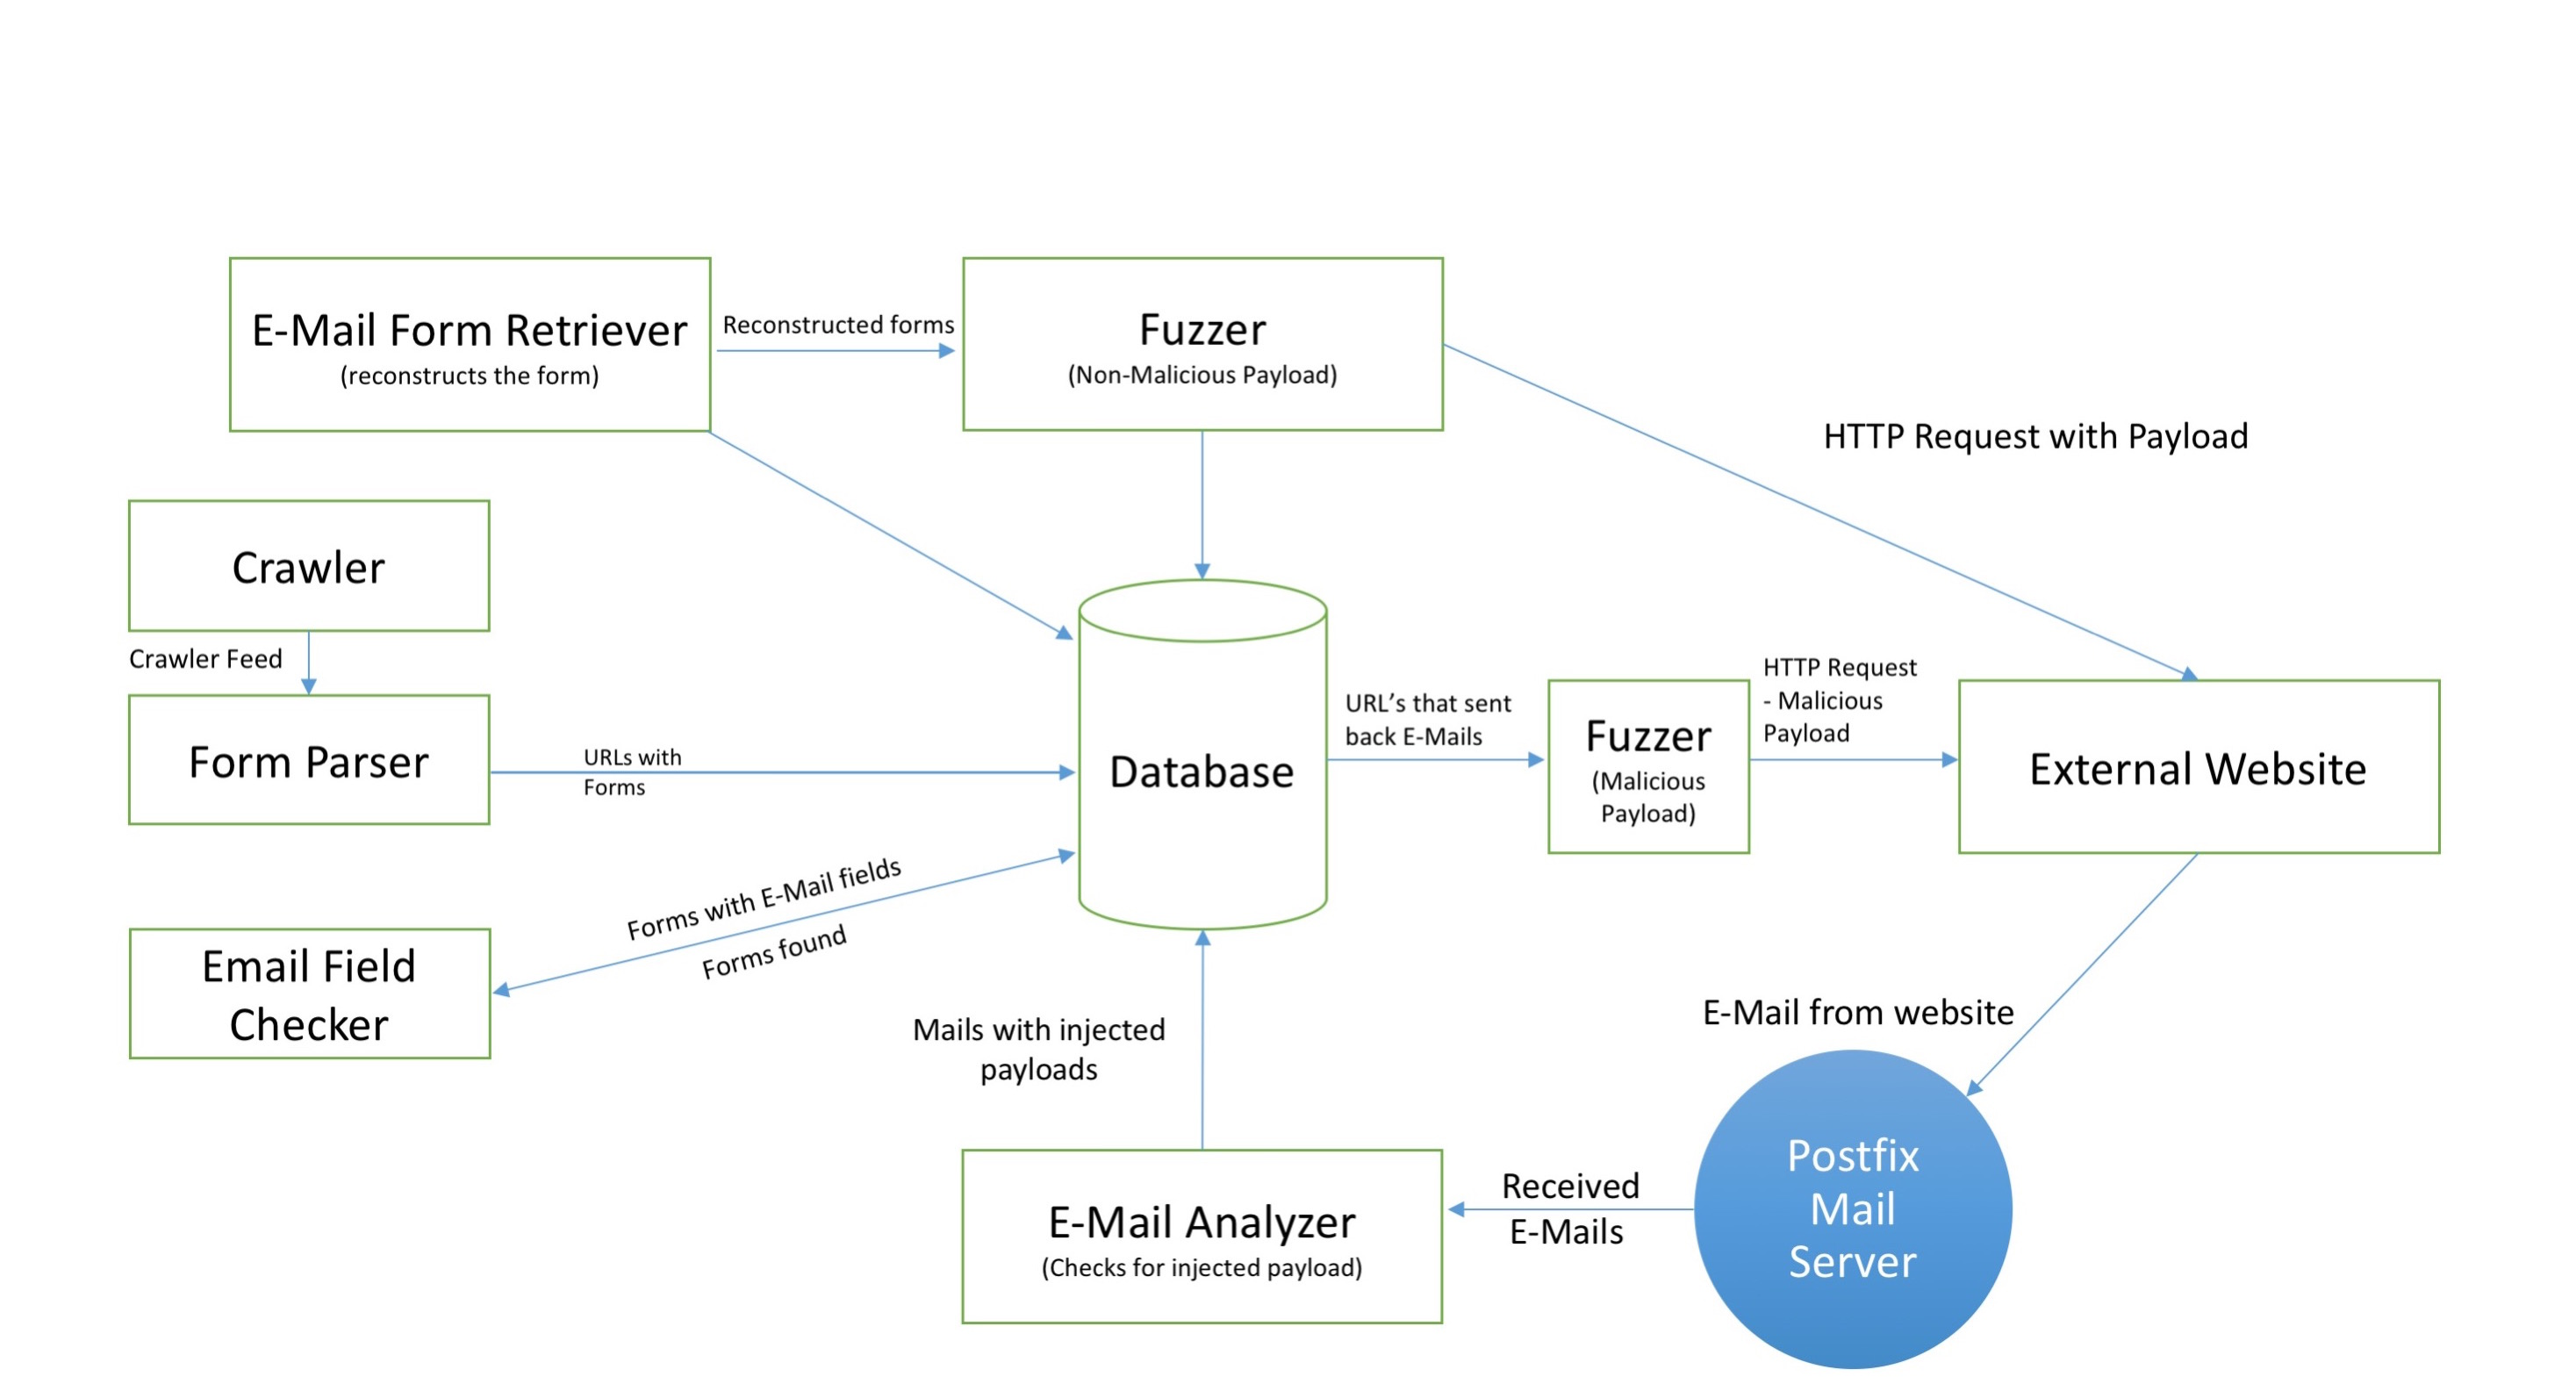
\includegraphics[width=.8\textwidth]{overall}
	\caption{Overall system architecture.}
	\label{fig:overall}
\end{figure*}

\subsection{System Architecture}
\label{sys:arch}
Our system can be broadly divided into two modules: Data Gathering and Payload Injection.

The Data Gathering module is responsible for the following activities:
	\begin{itemize}
		\item Interface with the Crawler (Section~\ref{Comp:Crawler}) and receive the URLs.
		\item Parse the HTML for the corresponding URL and store the relevant form data (Section~\ref{Comp:FP}).
		\item Check for the presence of HTML forms that could allow a user to send/receive \email and store references to these forms (Section~\ref{Comp:EMFC}).
	\end{itemize}
    
	The Payload Injection module is responsible for the following activities:
	\begin{itemize}
		\item Retrieve the HTML forms that could allow a user to send/receive \email and reconstruct these forms (Section~\ref{Comp:EMFR}).
		\item Inject these forms with benign data (non-malicious payloads) and generate an HTTP request to the corresponding URL (Section~\ref{Comp:Fuzzer:nmp}).
		\item Analyze the received \emails, extracting the \email header fields and checking for the presence of the injected payloads (Section~\ref{Comp:EMA}).
		\item Inject the HTTP requests that sent us \emails with malicious payloads, and generate an HTTP request to the corresponding URL to check if an \ehi vulnerability exists in that web application (Section~\ref{Comp:Fuzzer:mp}).
	\end{itemize} 
	%% The functionality of each component is discussed further in the `Components' section (Section~\ref{Comp}). The Payload Injection pipeline is not a linear, but cyclic process, as we inject different payloads and analyze the received \emails.


\subsection{System Components}
\label{Comp}

The Data Gathering module and Payload Injection modules are composed of smaller components. This section describes the functionality of each of the components.

\subsubsection{Crawler}
\label{Comp:Crawler}
We used an open-source Apache Nutch based Crawler~\cite{nutch}. The Crawler continuously crawls the web. The Crawler provides the system with a continuous feed of URLs and the HTML contained in those pages. 

\subsubsection{Form Parser}
\label{Comp:FP}
The actual analysis pipeline begins at the Form Parser. This module is responsible for parsing the HTML and retrieving data about the HTML forms on the page, including the following:
\begin{itemize}
	\item Form attributes, such as \texttt{method} and \texttt{action}. These dictate the resulting URL for the HTTP request and the method of the HTTP request.
	\item Data about the form input fields, such as their attributes, names, and default values. The default values are essential for fields like \colorbox{lightgray}{\lstinline{<input type="hidden">}} as these fields are usually used to check for the submission of forms by bots.
	\item Presence of the \colorbox{lightgray}{\lstinline{<base>}} element in the HTML, as this affects the final URL to which the form is to be submitted (if the \texttt{action} attribute is a relative URL).
      % Adam: this is not correct, the referrer header won't be used when we make the request. We will set the referrer header when we make the request to URL that the form is on
	%% \item Headers associated with the page, such as \texttt{referrer}. Once again, these were required to avoid the website from ignoring our system as a bot.
\end{itemize} 
The Form Parser stores all this data in our database, so as to allow the system to reconstruct all data necessary for fuzzing the web application.

\subsubsection{\Email Field Checker}
\label{Comp:EMFC}
The \Email Field Checker is the final stage in the Data Gathering module. It receives the output of the previous stage---HTML form data---and checks for the presence of \email fields in those forms. If any \email fields are found, it stores references to these forms.
The intuition here is that we do not want to try to fuzz all HTML forms on the web to look for \ehi vulnerabilities, rather just those HTML forms that are likely to invoke server-side email functionality.

The \Email Field Checker searches for the words \texttt{e-mail}, \texttt{mail} or \texttt{email} within the form, instead of an explicit HTML5 \email field (e.g.,\ \colorbox{lightgray}{\lstinline{<input type="email">}}). This is by design, taking into account a common design pattern used by web developers, where they may have a text field with an \texttt{id} or \texttt{name} attribute set to \texttt{email}, instead of an actual \email type attribute, for purposes of backward compatibility with older browsers.

%% Compared to searching for explicit \email fields, by searching for the presence of the words \texttt{\email}, \texttt{mail} or \texttt{email} in the form, we are assured very few false negatives. This is because our system is bound to find \email fields with their \texttt{type}, \texttt{name}, or \texttt{id} set to one of these words. The system is also substantially faster as we do not have to parse the individual form fields at this point in the pipeline. However, despite the advantages, this might also lead to a false positive rate. We discuss this possibility in detail in Section~\ref*{issues:fpr} - Design Issues.

The output of this stage is stored in the database for persistence and acts as the input to the Payload Injection module.

\subsubsection{\Email Form Retriever}
\label{Comp:EMFR}
The \Email Form Retriever is the first stage in the Payload Injection module. It has the following functions:
\begin{itemize}
	\item Retrieve new forms and ensure no duplication occurs before the fuzzing stage.
	\item Reconstruct each form, using the stored form data, specifically the input fields and their values.
	\item Construct the target URL for the \texttt{action} attribute of the form to create an HTTP request to the correct URL for fuzzing. 
\end{itemize}

\subsubsection{Fuzzer}
\label{Comp:Fuzzer}
% Adam: we should call these something else but modules. We already have the top two modules, which are composed of components, now we need to split these into something (not components again). - DONE
The Fuzzer is the only component that interacts directly with the external web applications. The Fuzzer is split into smaller parts, each of which is responsible for a particular type of fuzzing.  The system injects payloads in two stages: the goal is to reduce the total number of HTTP requests the system generates to detect an \ehi vulnerability. Making HTTP requests is an expensive process~\cite{httpperf}, and can cause bottlenecks in a Crawler-Fuzzer system~\cite{ShkapenyukTorstenSuel2001}.
The two different types of payloads used for fuzzing are:
\paragraph{Non-Malicious Payload}
\label{Comp:Fuzzer:nmp}
The regular or non-malicious payload is simply an \email address. The goal is to see if the web application will send an \email message based on our input. The specific format of the \email is \texttt{reguser(xxxx)@example.com}, where \texttt{xxxx} is replaced by an internal id that uniquely maps the payload to the form, and \texttt{example.com} is replaced by our domain.

\paragraph{Malicious Payload}
\label{Comp:Fuzzer:mp}
After receiving an \email from a specific form, we then use the malicious payload to try to exploit an \ehi vulnerability. We inject the form parameters with the \texttt{bcc} (blind carbon copy) header. If the vulnerability is present, this will cause the server to send a copy of the \email to the \email address we added as the \texttt{bcc} field.

We consider a special case: the addition of an \texttt{x-check:in} header field to the payloads. This is due to Python's exhibited behavior when attaching
headers. Instead of overwriting a header if it is already present, Python will ignore duplicate headers. So, if the \texttt{bcc} field is already present as part of the headers, our injected \texttt{bcc} header would be ignored. To overcome this, we inject a new header that is not likely to be generated by the web application. 

We created four different malicious payloads. Each of these payloads is crafted for a particular use case. The four payloads are:

\begin{enumerate}
	\item
	\texttt{nuser(xxxx)@example.com\textbackslash{}n\\bcc:maluser(xxxx)@example.com} 
	
	This payload is the most minimal payload: it injects a newline character followed by the \texttt{bcc} field.
	
	\item \texttt{nuser(xxxx)@example.com\textbackslash{}r\textbackslash{}n\\bcc:maluser(xxxx)@example.com}
	
	This payload is added for purposes of cross-platform fuzzing: \texttt{\textbackslash{}r\textbackslash{}n} is the ``Carriage Return - New Line (CRLF)'' used on Windows systems.~\cite{rfc2616}
	
	\item \texttt{nuser(xxxx)@example.com\textbackslash{}n\\bcc:maluser(xxxx)@example.com\textbackslash{}nx-check:in}
	
	As discussed previously, the addition of the \texttt{x-check:in} header is to inject Python-based web applications.
	
	\item \texttt{nuser(xxxx)@example.com\textbackslash{}r\textbackslash{}n\\bcc:maluser(xxxx)@example.com\textbackslash{}r\textbackslash{}nx-check:in}
	
	Same as the previous payload, but containing the additional \texttt{\textbackslash{}r} for Windows compatibility.
	
\end{enumerate}
The \texttt{(xxxx)} in each payload is replaced by an internal unique id to create a one-to-one mapping of the payloads to the forms.
% Adam: If we need to cut things for space, we can cut this next line and the payload coverage table.
The coverage provided by each payload is shown in Table~\ref{tab:payloadcov}.\\

\begin{table}[tbp]
	\centering
	\begin{tabular}{|c|c|c|}
		\hline
		\multicolumn{1}{|c|}{\textbf{Payload}} & \multicolumn{1}{c}{\textbf{Languages covered}} & \multicolumn{1}{|c|}{\textbf{Platforms covered}}\\
		\hline
		1 & PHP, Java, Ruby, etc. & Unix\\
		\hline
		2 & PHP, Java, Ruby, etc. & Windows\\
		\hline
		3 & Python & Unix\\
		\hline
		4 & Python & Windows\\
		\hline
	\end{tabular}
	\caption[\titlecap{Payload coverage}]{Payload coverage, each payload covers a different platform/language.}
	\label{tab:payloadcov}
\end{table}

Along with the payload, the Fuzzer also injects data into the other fields of the form. This data must pass validation constraints on the individual input fields (e.g.,\ for a name field, numbers might not be allowed).  As crawling and fuzzing input fields on the web is an open problem~\cite{raghavan2000crawling}, we chose to go with a best-effort approach. To maximize the amount of vulnerabilities the system discovers, the data injected into the input fields should adhere to the constraints. The Fuzzer uses a ``Data Dictionary'' which has predefined ``keys'' and ``values'' for standard input fields such as \texttt{name}, \texttt{date}, \texttt{username}, \texttt{password}, \texttt{text}, and \texttt{submit}.
% Adam: What does it mean here for these to be generated on-the-fly? Using templates? - Fixed.
The values for these are generated from the Data dictionary for each form, based on generally followed guidelines for such fields. For example, password fields should consist of at least one uppercase letter, one lowercase letter, and special characters.
% Adam: can you add a sentence here about crawling and fuzzing fields on the web is an open problem (and cite ``Crawling the hidden web'' - DONE.

When the fuzzed data is ready, the Fuzzer constructs the appropriate HTTP request (GET or POST) and sends the HTTP request to the URL that was generated by the \Email Form Retriever (Section~\ref{Comp:EMFR}). 


\subsubsection{Injection Verification}
\label{Comp:EMA}
The Injection Verification module checks for the presence of injected data in the received \emails. This module works on the \emails received and stored by our Postfix server, and, depending on the user account that received the \email, it performs different functions.
\paragraph{Analyzing regular e-mail}
\sloppy
`Regular \email' refers to the \emails received by account \colorbox{lightgray}{\lstinline{reguser(xxxx)@example.com}} that were sent due to injecting the regular, non-malicious, payload (discussed in Section~\ref{Comp:Fuzzer:nmp}). The objective of the analysis on this \email is identify if the input fields that we injected with data appear on the resulting \email, and if so, which fields appear where.

To find this, we parse each received \email, and check whether \emph{any} of the fields we injected with data appear as part of either the headers or the body of the \email. If they do, we add them to the list of fields that can potentially result in an \ehi vulnerability for the given \email. We then pass on this information back to the Fuzzer pipeline, along with the vulnerable form.

\paragraph{Analyzing \email with payloads}
The ``\emails with payloads'' refers to \emails received by either the \colorbox{lightgray}{\lstinline{nuser(xxxx)@example.com}} or \colorbox{lightgray}{\lstinline{maluser(xxxx)@example.com}} accounts. These \emails could only be received as a result of injecting the malicious payloads that were discussed in Section~\ref{Comp:Fuzzer:mp}. 

\paragraph{Detecting injected \texttt{bcc} headers}
As discussed in the payloads section~(\ref{Comp:Fuzzer:mp}), the payloads were crafted such that the \emails received by the \texttt{maluser} account directly indicate the presence of the injected \texttt{bcc} field. 

\label{analyze:detect_x_check}
\paragraph{Detecting injected \texttt{x-check} headers}
\Emails not received by the \texttt{maluser} account but by the \texttt{nuser} account constitute a special category of \emails.
These \emails could have been generated due to two reasons:
\begin{enumerate}
	\item The web application performed some sanitization routines and stripped out the \texttt{bcc} part of the payload, thereby sending \emails only to the \texttt{nuser} account. These \emails then act as proof that the vulnerability was not found on the given URL.
	\item The \texttt{bcc} header can be ignored for other reasons (e.g.,\ Python's default behavior when it encounters duplicate headers). In this case, we check if the \email contains the custom header \texttt{x-check}. If it does, then this is a successful exploit of the vulnerability.
\end{enumerate}



\section{Implementation}

Our system was run on a server with the following configuration: Dell
PowerEdge T110 II Server, CPU: Intel(R) Xeon(R) CPU E3-1220 V2 @
3.10GHz, Cache Size: 8,192 KB, No. of Cores : 4, Total Memory (RAM) : 16 GB.

\subsection{Validation}
To validate our system, we constructed three sets of web applications in PHP, Python, and Ruby. Each of these applications was a simple web application that accepted user input to construct and send an \Email.

The front-end for each of the three applications is shown in Listing~\ref{code:html}. The server-side code for PHP, Python, and Ruby is shown in Listings~\ref{code:phpemi}, \ref{code:pyemi}, and \ref{code:rubyemi} respectively.

% Adam: I think it might be nice to have the Ruby code here too. - DONE.

Before performing a wide scan of the web, we verified that our system was able to detect the \ehi vulnerabilities present in all the sample web applications. 

%% We tested for the headers being injected in real-time by running an instance of MailCatcher, set to listen on all SMTP messages. A sample screenshot of a fuzzed request for the Ruby backend (generated in PostMan) is shown in Figure~\ref{fig:postmanruby}. The \email sent due to injecting this payload (as captured by MailCatcher) is shown in Figure~\ref{fig:mailcatcherruby}. It can be seen that the headers have been added to the resulting \email, and we have successfully managed to overwrite the \texttt{Subject} field with our message, `hello'.

%% The astute reader might have noticed that in the given example we have used \texttt{\%0a} to separate the headers, while in Section~\ref{Comp:Fuzzer:mp}, we had used \texttt{\textbackslash{}n}. This is due to URL encoding~\cite{rfc1738}, wherein special characters in th URL are `encoded' or `escaped' with their ASCII equivalent.
%% The reason why we do not have to do this with the payloads our system injects is due to the fact that the Python Requests library that we use to generate the HTTP requests automatically does this encoding for us.

\begin{lstlisting}[language=HTML,caption={HTML page for showcasing
      \ehi, a simple front-end for our
      examples.},label={code:html}, float]
<!doctype html>
<html lang="en">
<head>
<meta charset="utf-8">
<meta name="author" content="XYZ">
<title>Mock Email</title>
</head>
<body>
<form action="{path-to-back-end}" method="post">
<input type="text" placeholder="Email" name="email" id="\email"><br>
<textarea name="msg" rows="20" cols="120"></textarea>
<input type="submit" value="Email Me!">
</form>
</body>
</html>
\end{lstlisting}
\begin{lstlisting}[language=Ruby,caption={Ruby program with e-mail
      header injection vulnerability.},label={code:rubyemi}, float]
require 'sinatra'
require 'net/smtp'

get '/hello' do
email = params[:email]

message = """
From: Sch <sch@example.com>
Subject: SMTP e-mail test
To: #{email}

This is a test e-mail message.
"""
# construct a post request with email set to attack_string
# attack_string => s@example.com%0abcc:spc@example.com%0aSubject:Hello
Net::SMTP.start('localhost', 1025) do |smtp|
smtp.send_message message, 'sch@example.com',
'to@todomain.com'
end
# Headers get added, and Subject field changes to what we set.
end
\end{lstlisting}


%% \begin{figure}[tbp]
%% 	\centering
%% 	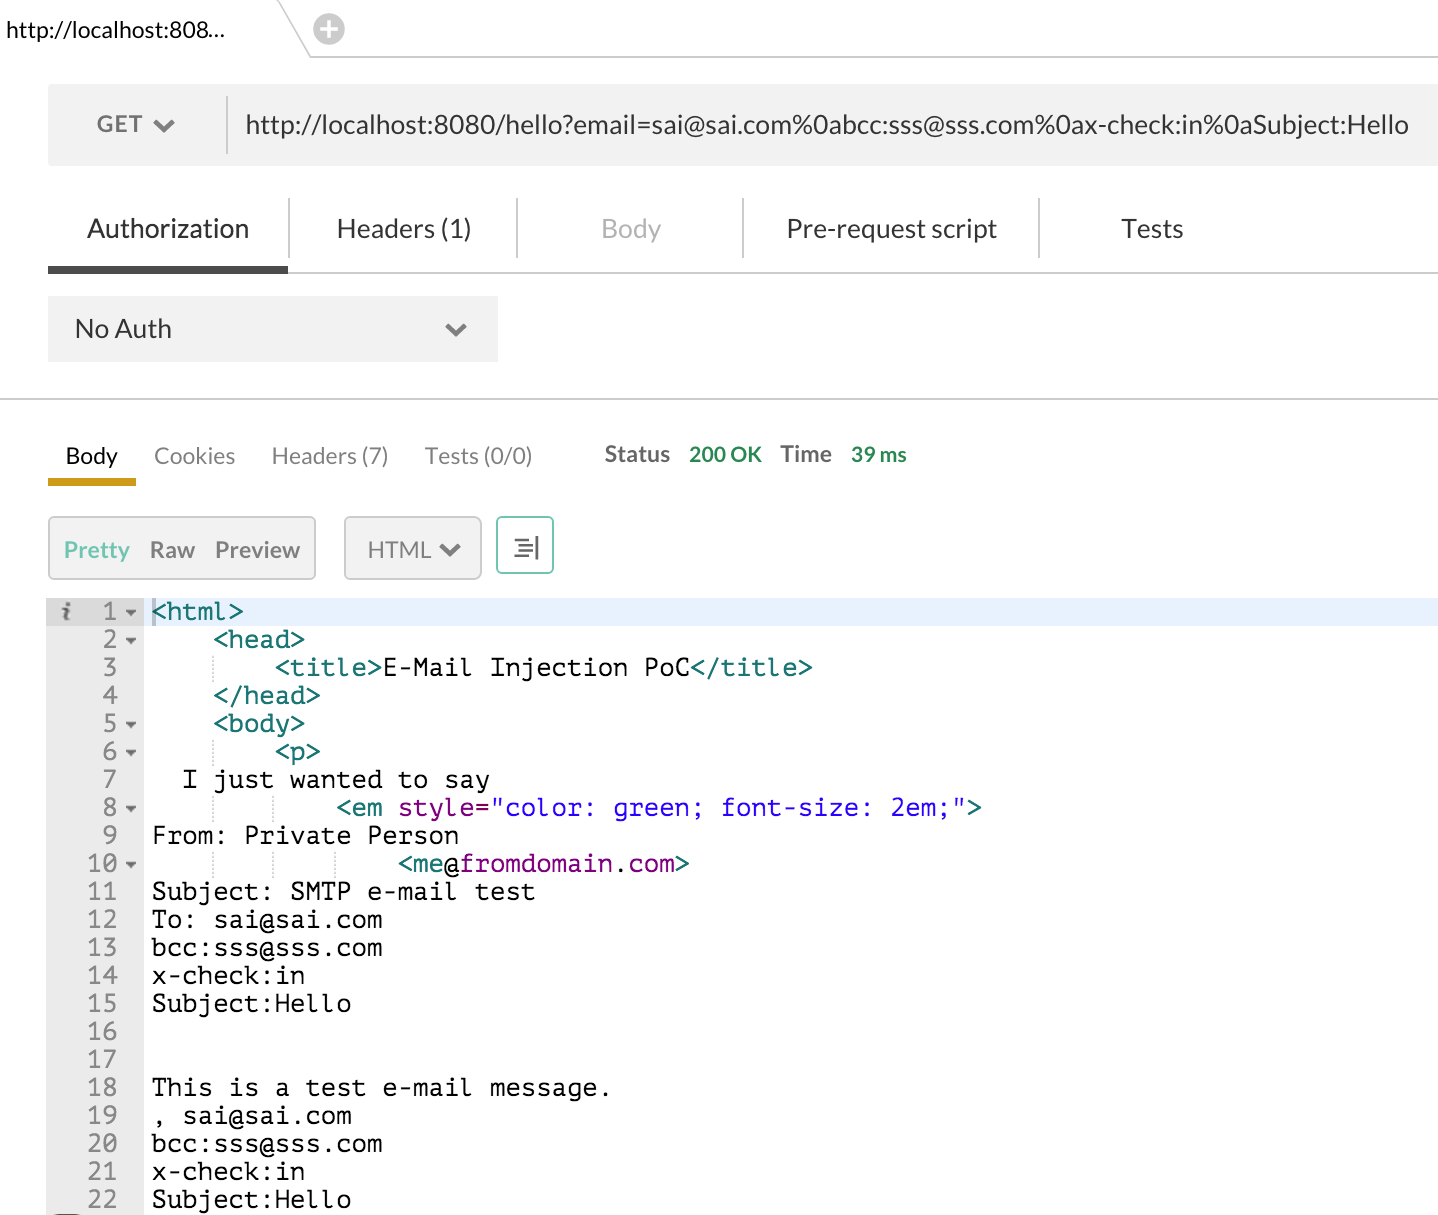
\includegraphics[width=\linewidth]{System/EMI_Postman_Ruby}
%% 	\caption[\titlecap{Fuzzing a request for the Ruby backend}]{Fuzzing a request for the Ruby backend, the payload can be seen inside the address bar.}
%% 	\label{fig:postmanruby}
%% \end{figure}

%% \begin{figure}[tbp]
%% 	\centering
%% 	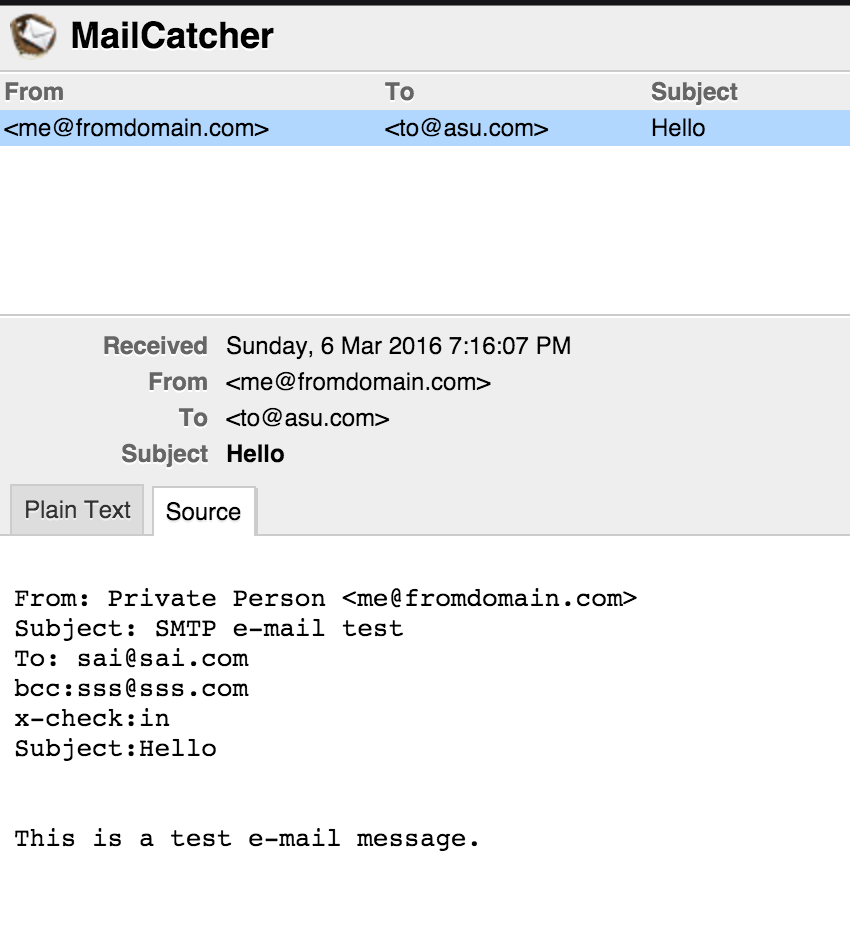
\includegraphics[width=\linewidth]{System/EMI_Mailcatcher_Ruby}
%% 	\caption[\titlecap{\Email Header Injection proof of concept - Ruby}]{\Email header injection proof of concept - Ruby, we can see that multiple headers (bcc, x-check, subject) have been inserted into the resulting \email.}
%% 	\label{fig:mailcatcherruby}
%% \end{figure}


\section{Evaluation}

We ran our system on the web at large, attempting to discover \ehi vulnerabilities in web applications. 
\subsection{Collected Data}

% TODO: Need to put in a number here, and discuss the high level
% crawl. - DONE

From our extensive crawl of the web, we were able to gather the data
shown in Table~\ref{tab:data}. We ran the system for 76 days, during which our system crawled \urls unique URLs,
and found a total of \forms\ forms from \uniqueforms\ unique domains. Out of these forms, our system
found \emailforms\ forms that contained an \email field, from \uniqueemailforms\ unique domains.

\begin{table}[tbp]
	\centering
	\begin{tabular}{|c|c|}
		\hline
		\multicolumn{1}{|c|}{\textbf{Type of Data}} &
		\multicolumn{1}{c|}{\textbf{Quantity}}\\
		\hline
		URLs Crawled & \urls \\
		\hline
		Total Forms found & \forms \\
		\hline
		Forms with E-Mail Fields & \emailforms \\
		\hline
	\end{tabular}
	\caption[\titlecap{Collected data}]{The data collected for our project.}
	\label{tab:data}
\end{table}



\subsection{Fuzzed Data and Received \Emails}
Table~\ref{tab:fuzzed_data} shows the quantity of \emails that we received for the benign and malicious payloads. 
\begin{table}[tbp]
	\centering
	\begin{tabular}{|c|c|c|}
		\hline
		\multicolumn{1}{|c|}{\textbf{Type of fuzzing}} &
		\multicolumn{1}{c|}{\textbf{Forms fuzzed}} &
		\multicolumn{1}{c|}{\textbf{E-Mails received}}\\
		\hline
		Regular payload & \fuzzed & \recd \\
		\hline
		Malicious payload & \malfuzzed & \success \\
		\hline
	\end{tabular}
	\caption[\titlecap{Fuzzed data}]{The data that we fuzzed and the e-mails that we received.}
	\label{tab:fuzzed_data}
\end{table}

\paragraph{\Email received from forms}
The \emails that we received can be categorized into two categories:
\begin{enumerate}
	\item \Emails due to regular payload\\
	This represents the total number of web applications that sent \emails to us. This indicates that we were able to successfully submit the forms on these sites to trigger the web application to send an \email.
	
	\item \Emails due to malicious payload\\
    Once we receive an \email from a web application due to the regular payload, we fuzz those forms with the malicious payloads. This field represents the total number of unique URLs that are  contain an \ehi vulnerability.
\end{enumerate}




\subsection{Analysis of the Received \Email Data}
During our analysis of the received \emails, we found that the \emails that we received belonged to one of three categories:
\begin{enumerate}
	\item \Emails with the \texttt{bcc} header successfully injected\\
	  This form of injection was our initial objective, and we found
% Adam: Sai, why isn't this number a command? - DONE.
      \ehibcc such \emails in our received \emails. This validates that the web applications that sent these \emails are vulnerable to \ehi.
	
	\item \Emails with the \texttt{to} header successfully injected\\
	We discovered an unintended vulnerability class during our analysis, which we call \texttt{To~header injection}. These injections reflect the ability to inject any number of \email addresses into the \texttt{to} field of the SMTP message while being unable to inject any other header into the \emails. We found \ehito such \emails in our received \emails. We attribute this behavior to inconsistent sanitization by the application. 
    % Adam: I can't understand what this sentence is trying to say - Removed.
	
	While not allowing us complete control over content of the \emails sent, \texttt{To header injection} makes it possible to append any number of \email addresses, thereby enabling us to leak information or perform DoS (Denial of Service) attacks against the web application.
	
	\item \Emails with the \texttt{x-check} header successfully injected\\
    The third category of \emails received were \emails with the \texttt{x-check} header injected. As discussed in Section~\ref{analyze:detect_x_check}, 
    we can differentiate between unsuccessful attempts and successful attempts by injecting the additional header and checking whether headers other than the \texttt{bcc} header can be injected into the generated \email. \ehixcheck \emails were received with the \texttt{x-check} header injected.
\end{enumerate}

% Adam: Sai, we need to put the actual numbers in the text. We cannot count on the readers to look at the table (of course, we should use the commands
We list each category and the number of \emails received by that category in Table~\ref{tab:analysis}. 
We explain the combination of these header injections (4-7) as follows:

\begin{table*}[tbp]
	\centering
	\begin{tabular}{|l|c|}
		\hline
		\multicolumn{1}{|c|}{\textbf{Type of Injection}} &
		\multicolumn{1}{p{3cm}|}{\centering \textbf{No. of e-mails received}}\\
		\hline
		E-Mail Header Injections with \texttt{bcc} header & \ehibcc \\
		\hline
		E-Mail Header Injections with \texttt{x-check} header & \ehixcheck \\
		\hline
		\texttt{To header} injections alone & \ehito \\
		\hline
		E-Mail Header Injections with \texttt{bcc} and \texttt{x-check} headers & \ehibccxcheck \\
		\hline
		Both \texttt{To header} injections and x-check headers &
		\ehitoxcheck \\
		\hline
		\texttt{x-check} headers found in \texttt{nuser} e-mails & \ehinuserxcheck \\
		\hline
		Unique \texttt{x-check} headers found in \texttt{nuser} e-mails & \ehiuniquenuserxcheck \\
		\hline
		Total successful injections (1 + 3 + 7) & \success \\
		
		\hline
	\end{tabular}
	\caption[\titlecap{Analysis of the data}]{Classification of the e-mails that we received into broad categories of the vulnerability.}
	\label{tab:analysis}
\end{table*}


\begin{itemize}
	\item \Email Header Injections with both \texttt{bcc} and \texttt{x-check} headers\\
	  These represent the scenario where an attacker can inject multiple headers into the \emails. We can see that 65.65\% of the received \texttt{bcc} header injected \emails are also susceptible to being injected with additional headers.
      % Adam: What is the exact percentage? We should use that rather than an approximate number - DONE.
	
	\item Both \texttt{To} header injections and \texttt{x-check} headers \\
	This combination shows us that in addition to being able to inject into the \texttt{To} fields, we injected additional headers into the \email. It is not clear what causes this behavior; however, these can be exploited to achieve the same result as a regular \ehi.
	
	\item Total \texttt{x-check} headers and unique \texttt{x-check} headers found in \texttt{nuser} \emails\\
		We found a total of \ehinuserxcheck \emails in the \texttt{nuser} account. Out of these, \ehiuniquenuserxcheck had unique form ids that were \emph{not} already found in the \texttt{maluser} account. We attribute these \emails to (probably) being sent by a web application that was built with Python or another language having a similar behavior with respect to ignoring duplicate headers while constructing an \email, thus appending the \texttt{x-check} header and \emph{not} the \texttt{bcc} header. 
      % Adam: What is the actual behavior? This is confusing. - Changed. DONE.
	
	\item Total successful injections\\
	  This represents the total number of successful injections. This includes the \ehi with \texttt{bcc} header\,(1), \texttt{To} header injections alone\,(3), and Unique \texttt{x-check} headers found in \texttt{nuser} \emails\,(7). A total of \success vulnerabilities were found by our system.

      % Adam: we need the actual #s here too. These are the core results of our analysis, they need to be in the text. - DONE.
	
\end{itemize}

\subsection[The Pipeline]{Understanding the Data Pipeline}
%This section serves to represent our pipeline quantitatively and graphically. 
Table~\ref{tab:pipeline} showcases the data gathered by our pipeline, with the differential changes at each stage of the pipeline. 

At each stage of the pipeline, the amount of data decreases, for instance, out of the \urls\ URLs we crawled, only \forms\ forms (\formsDelta) were found. Out of these, only \emailforms\ forms (\emailformsDelta) contained e-mail fields.

In our fuzzing attempts, the same behavior is repeated. We fuzzed \fuzzed\ forms with the regular payload, which resulted in a total of \recd\ e-mails (\recdDelta). After analysis of the received e-mails, we further fuzzed \malfuzzed\ forms, which resulted in \success\ e-mails (\successDelta) which contain the vulnerability across \ips IP Addresses corresponding to \domains domains.

The reason for the difference in the number of forms found and the number of forms fuzzed is discussed in the Limitations section~(\ref{limitations}).

\begin{table*}[tbp]
	\centering
	\begin{tabular}{|l|c|c|}
		\hline
		\multicolumn{1}{|c|}{\textbf{Pipeline Stage}} &
		\multicolumn{1}{p{3cm}|}{\centering \textbf{Quantity}} &
		\multicolumn{1}{p{2.8cm}|}{\centering \textbf{Differential}
		$\Delta$ d2/d1 * 100}\\
		\hline
		Crawled URLs  & \urls &  --- \\
		\hline
		Forms found  & \forms & \formsDelta \\
		\hline
		E-Mail Forms found  & \emailforms & \emailformsDelta \\
		\hline
		Fuzzed with regular payload  & \fuzzed & \fuzzedDelta \\
		\hline
		Received e-mails  & \recd & \recdDelta \\
		\hline
		Fuzzed with malicious payload  & \malfuzzed & \malfuzzedDelta \\
		\hline
		Successful attacks  & \success & \successDelta \\
		\hline

	\end{tabular}
	\caption[\titlecap{Data gathered by our pipeline}]{Data gathered by our pipeline at each stage, with the differential between the stages.}
	\label{tab:pipeline}
\end{table*}



% Adam: this is an important part of our contribution, but I don't think that it belongs here. 
%% From our research, it is clear that E-Mail Header Injection is quite widespread as a vulnerability, appearing on \successDelta\ of forms that we were able to perform automated attacks on. This value acts as a lower bound for E-Mail Header Injection vulnerability, and can quite easily be much more if the attacks were of a more concentrated nature, crafted for the individual websites and less automated.

\subsection{Responsible Disclosure of Discovered Vulnerabilities}
After we discovered an \ehi vulnerability on a particular website, we attempted to notify the developers of the vulnerable web application, along with a brief description of the vulnerability.
We chose to \email the following mailboxes, following the rules specified in RFC~2142~\cite{rfc2142}:
% Adam: don't we use \texttt for all the email addresses in the paper? We should use the same thing here - DONE.
\begin{itemize}
	\item \texttt{security@domain.com} - Used for Security bulletins or queries.
	\item \texttt{admin@domain.com} - Used to contact the administrator of a website.
	\item \texttt{webmaster@domain.com} - Synonym for administrator, same functionality as admin.
\end{itemize}

% Adam: sai, is this number up-to-date? 
Out of the \domains\ vulnerable domains found, only \emailedDefaultmailbox websites had the mailboxes able to receive \emails. For the remaining domains, we used the \texttt{whois}~\cite{whois} data to find the contact details of the owner and then \emailed them. The number of emails we sent and the number of developer responses we received is shown in Table~\ref{tab:devresp}.

\begin{table}[tbp]
\centering
\normalsize
\begin{tabular}{|c|c|c|}
	\hline
	\multicolumn{1}{|p{2cm}}{\centering \textbf{Notified websites}} &
	\multicolumn{1}{|p{2cm}|}{\centering \textbf{Developer Responses}} &
	\multicolumn{1}{p{2cm}|}{\centering \textbf{Confirmed discoveries}}\\
	\hline
	\domains\ & \responses & \confirmed \\
	\hline
\end{tabular}
	\caption[\titlecap{}]{Responsible disclosure of the discovered vulnerabilities to developers and the number of received responses.}
	\label{tab:devresp}
\end{table}

% Adam: did we get updated notifications? - nope. DONE.
We received \responses developer responses, confirming \confirmed discovered vulnerabilities. Three of the developers fixed the vulnerability on their website.
% is this done? 1 additional email asking for more information, but no confirmation.
From our research, it is clear that \ehi is quite widespread as a vulnerability, appearing on \successDelta\ of forms that we were able to perform automated attacks on. This value acts as a \emph{lower bound} for prevalence of \ehi vulnerability, and can quite easily be larger if the attacks were broader, crafted for the individual web application, and  less automated. 

\subsection{Exploitation Evidence}
We compared the \ips IPs that our system found to be vulnerable to \ehi against 13 well-known IP blacklists, to see if these IPs were being exploited by attackers to send spam. The blacklists that we used were: 
\texttt{zen.spamhaus.org},
\texttt{spam.abuse.ch},
\texttt{cbl.abuseat.org},
\texttt{virbl.dnsbl.bit.nl},
\texttt{dnsbl.inps.de},
\texttt{ix.dnsbl.manitu.net},
\texttt{dnsbl.sorbs.net},
\texttt{bl.spamcannibal.org},
\texttt{bl.spamcop.net},
\texttt{dnsbl-1.uceprotect.net},
\texttt{dnsbl-2.uceprotect.net},
\texttt{dnsbl-3.uceprotect.net},
\texttt{db.wpbl.info}

We found that \ipsblacklist of these IPs were blacklisted on at least one of the above blacklists for sending out spam, and \ipsblacklistmulti of them were found on multiple blacklists. We do not have enough data to make an observation about whether these attackers are exploiting \ehi to send out the spam, as an alternative hypothesis is that these IPs are on the blacklists because the server has different vulnerabilities that attackers exploit to cause the server to send spam (assuming that the server is normally benign).  



\section{Discussion}
    In this section, we discuss the lessons learned, the limitations of our system, and how to mitigate \ehi vulnerabilities.
\subsection{Lessons Learned}
From our results, it is evident that \ehi vulnerabilities exist in the wild.
% Adam: Sai, I don't understand this math. The 1.46% number is calculated based on the number of forms we were able to fuzz with a malicious payload. This isn't the same as the number of websites. But, using 673/21675680 is not good either because that is # of URLs and it seems like the number you have here is websites. What we need is what % of *websites* (probably estimated as domains) did we find to be vulnerable out of *all* websites/domains that we found. When we use this number, we need to be clear what it is that we are using. -- FIxed this to be clear.
Despite its relatively low occurrence rate compared to the more popular SQL Injection and XSS (Cross-Site Scripting), when we consider total number of domains on the World Wide Web--- 1,018,863,952 according to Internet Live Stats~\cite{InternetLiveStats2016} as of early 2016---and calculate \successWebsitesDelta percent (the occurrence rate of \ehi vulnerability calculated from vulnerable domains as found by our system to total number of domains crawled) of that number, this yields 295,693 domains. Of course, extrapolation in this way is not an accurate measure of the prevalence of \ehi vulnerabilities. However, even with as few as a thousand domains affected by this vulnerability, it can still have a disastrous impact on these domains, and also on overall World Wide Web due to the traffic caused by the sheer number of generated e-mails. 
    
%% We believe that one of the reasons for the small percentage of occurrence (compared to SQL Injection or Cross-Site Scripting), can be attributed to what we like to call the `car parking analogy'.
%%     The car parking analogy is something like this: Imagine that we are parking a car on a road that is prone to attacks by thieves. Now, if all the cars were unlocked, the car that is most likely to get stolen is quite unsurprisingly the most expensive one or the one that is easiest to get away with.
    
%%     Now imagine the same thing on the World Wide Web: we have websites that can each have multiple vulnerabilities. Now, it makes sense for an attacker to try and attack websites with more widespread vulnerabilities such as SQL Injection or XSS, rather than attempt to exploit E-Mail Header Injection, seeing as this requires a more concentrated effort, with carefully crafted payloads and a waiting time for the e-mail to be delivered. SQL Injection attacks and XSS attacks are also better documented, with well-known attack vectors, and automated tools to help detect the presence of these vulnerabilities on websites.
    
%%     This also gives more incentive for the website developer to add protection against attacks such as SQL injection and XSS. The developer might then (possibly with the help of a sanitization library) sanitize the user input and remove \emph{all} special characters, including the newline characters (\textbackslash{}n, \textbackslash{}r), which adversely affects E-Mail Header Injection attacks.

%% 	We come to this conclusion because of our discovery of the \texttt{To header injection}. Clearly, this is possible due to incomplete sanitization performed by the application. We suspect that this incomplete sanitization is actually sanitization that is performed for some other vulnerability, and not specifically for E-Mail Header Injection attacks. We would also like to remark that \texttt{To header injection} is not complete E-Mail Header Injection, but only a special subset.
	
%%     Thus, indirectly, this kind of protection against other attacks affects the attempts to perform E-Mail Header Injection. However, this does not completely negate the attempts if the checks are only on the client-side. Also, even with server-side validation, often, the only input fields that are validated are ones that are either inserted into the database (SQL Injection) and the ones that are displayed to the user as part of the web site (XSS).

% Adam: Please add a citation to a CAPTCHA paper - DONE.
	A common reason for our fuzzing attempts to fail is the bot-blocking mechanisms built into the web applications. CAPTCHAs (Completely Automated Public Turing test to tell Computers and Humans Apart)~\cite{captchas2} pose a very difficult problem for our system to exploit \ehi, even if it is present.

	%% This does not mean that the vulnerability is not a large threat. In fact, this vulnerability can also have some major consequences, the least of which can be spamming and phishing attacks.
	%% In today's digital world, identity theft has become all the more common. E-Mail Header Injection provides attackers with the ability to easily extract information about users, not just from a server, but from the user himself, by sending him fake messages that look extremely authentic, since these messages are sent by the mail server of the website itself.
    
    We found two different forms of \ehi: the first one is the traditional one, injecting any header into the \email that allows the attacker complete control over the contents of the \email. 
The second attack has not yet been documented and provides the ability to inject multiple \email addresses into the \texttt{To} field. We call this a \texttt{To header injection}. In this  vulnerability, an attacker can add addresses to the \texttt{To} field of the email with newlines separating the \email addresses. We could not determine if this vulnerability is due to unique flaws in each web application or if this vulnerability is due to an implementation issue with a particular language or framework. However, from our preliminary analysis, it is evident that the vulnerable web applications do not share much in common. 

\texttt{To header injection} allows an attacker to extract information that should be private,
% Adam: It's not clear what this means that we have enough data to spoof the few lines of the message. I thought to header injection just controls the TO field, not the message contents. - Fixed, my bad. DONE.
and in some of these cases, able to inject enough data to spoof other headers of the \email message. From Table~\ref{tab:analysis}, information leakage using \texttt{To header injection} was possible on \ehito forms, while spoofing using \texttt{To header injection} was possible on \ehitoxcheck forms.
    
    %% While not being as impactful as the primary vulnerability, this form of the vulnerability does still provide the ability to send \emails to multiple recipients, and can easily result in information leakage or spam generation on a large scale.
    

\subsection[Limitations]{Limitations}
\label{limitations}
		Because our system is fully automated, it is also susceptible to being stopped by mechanisms in web applications that prevent automated crawls or form submissions. Measures such as CAPTCHA, hidden form fields and CSRF (Cross-site Request Forgery~\cite{csrf}) tokens are often used to detect bots~\cite{captchas3, captchas2}.

		We made sure that we do not fuzz hidden fields in the form, and because our system does not depend on authenticated sessions, CSRF tokens do not pose an issue. However, despite considerable active research in breaking CAPTCHAs~\cite{captchas2, captchas}, breaking CAPTCHAs remains out of the scope of this project. 
		
	   Due to the growing emphasis on responsive web applications, more and more web applications are being built with only client-side JavaScript. Even conventional web applications use JavaScript to dynamically insert content and update the pages. This trend means that these dynamically injected HTML components are not part of the initial HTML that is sent to the client by the server.

		Thus, our system will not see dynamically injected forms and hence is unable to detect whether \ehi vulnerabilities are present in these forms. The workaround would be to use a JavaScript engine to query for the \texttt{document.getElementsByTagName('html')[0].innerHTML} (from inside web browser automation tools such as Selenium), then use that as the source HTML. 
		
		%TODO Adam: added a table here, and explanation about performance tradeoffs with Selenium and bs4.
		A comparison of the running times between the different approaches is shown in Table~\ref*{tab:perf}. Because using Selenium results in a slowdown of \slowSelenium, we chose not to do this for performance reasons. 
		
		\begin{table}
			\centering
			\normalsize
			\begin{tabular}{|p{4cm}|c|c|}
				\hline
				\multicolumn{1}{|c}{\textbf{Method}} &
				\multicolumn{1}{|c|}{\textbf{Running time}} &
				\multicolumn{1}{|c|}{\textbf{Slowdown}}
				\\
				\hline
				\centering Using our pipeline & 629.043 & - \\
				\hline
				\centering Adding Selenium to our pipeline & 919.372 & \slowSelenium \\
				\hline				
				\centering Detecting \email fields by parsing each field instead of `grep'ing inside form & 707.154 & \slowParse \\								
				\hline
			\end{tabular}
			\label{tab:perf}
			\caption[\titlecap{}]{Running times in seconds for crawling, parsing, and detecting presence of \email fields in 1000 random wikipedia pages.}
		\end{table}

        Because we search for the words \texttt{e-mail}, \texttt{mail}, or \texttt{email} within the HTML form, if the website does not use English names for its forms our system will not be able to find the presence of an \email field. An example is shown in Listing~\ref{code:htmlfrench}. Here, the French word for \texttt{e-mail}---courrier électronique---is used, and our system is unable to find the presence of the e-mail field. 
        
		During the crawl, our system was blacklisted by a few web applications (mostly WordPress ones), and Internet Service Providers (ISPs).
		To overcome this, we did two things:
		\begin{enumerate}
			\item Used an IP range of 60 different IP addresses.
			\item Used a blacklist of our own to prevent our Fuzzer from fuzzing web application that are known to blacklist automated crawlers.  However, we could not gather any data about these web applications.
		\end{enumerate}

		We found that certain WordPress plugins prevent the \ehi attack by sanitizing user input on contact forms. Although not all  WordPress web applications are secure, between the presence of the plugins on some websites, and getting tagged as ``spambots'' by others, we found few vulnerabilities on WordPress web applications.

        E-Mail libraries such as the PHP Extension and Application Repository's (PEAR) mail library provide sanitization for user input. While this is not strictly a limitation of our project, it still means that we are not able to inject sites that used these libraries successfully.

        The parser that we use for HTML parsing---Beautiful Soup---does not parse malformed HTML and throws an exception on encountering malformed HTML. Thus, we have designed the system to exit gracefully on such occasions. A side-effect of this is that our system is unable to test web applications with bad HTML markup\,\footnotemark.

        \footnotetext{We do not have any data about whether bad markup indicates an overall lower quality of the web application, and thus cannot comment on whether such websites are more likely to have vulnerabilities.}

        Black-box testing is highly beneficial as explained in Section~\ref{sys:appr}, however it also has a drawback in that we cannot verify whether the reported vulnerability exists in the source code or is a feature of the website (e.g., the website allows users to send bulk e-mail, adding as many \texttt{cc} or \texttt{bcc} headers). We must manually notify the developers to get this feedback.

%%        	As discussed in Section~\ref{Comp:EMFC}, we only search for the words \texttt{email}, \texttt{mail} or \texttt{e-mail} (case insensitive) inside the forms to detect the presence of e-mail fields, instead of searching for an \colorbox{lightgray}{\lstinline{<input type = email>}}. This might result in a false positive in certain forms, like the one shown in Listing~\ref{code:false_positive}.

%%        	\begin{lstlisting}[language=HTML,caption={E-Mail field checker
%%               - false positives, the system incorrectly classifies
%%               this as an e-mail form.},label={code:false_positive}, float]
%% <form method="post">
%% E-Mail us if you have any questions!!
%% <input type="text" name="query"><br>
%% <input type="submit" value="Search">
%% </form>
%%        	\end{lstlisting}

%%        	The word \texttt{E-Mail} on Line 2 will result in our system classifying this form as a potential e-mail form, while it clearly is not. However, as we will see, this is not really a significant issue, as despite being added to the \texttt{email\_forms} table, this form will never be injected in the `fuzzer' due to the absence of the appropriate input field in the form. We chose to go with this design, as it allows us to detect almost every form that provides the capability to send or receive e-mail.

\begin{lstlisting}[language=HTML,caption={e-mail field in a different language - French.},label={code:htmlfrench}, literate=%
	{é}{{\'e}}1, float]
<input type="text" 
placeholder="courrier électronique"
name="courrier_électronique">
\end{lstlisting}

\subsection{Assumptions}
In addition to the limitations that were already discussed, we made certain assumptions while building the system. This section describes the assumptions and explores to what extent these hold true:
\begin{enumerate}
	\item \textbf{The crawler is not blocked}\\
	This is a requisite for our system to work. If the Crawler is blocked for any reason, we do not get the data feed for our system, and without this input, it is impossible to discover vulnerabilities. 
	
	\item \textbf{The Crawler feed is an ideal representation of the World Wide Web} \\
	This is a reasonable expectation, albeit an unrealistic one.
It is unrealistic because Crawlers work on the concept of proximity. They detect for the presence of In-Links and Out-Links from a particular URL, and hence the returned URLs are usually related to each other (at least the ones that are returned adjacent to each other).	However, this assumption is reasonable due to the ``Law of averages''~\cite{wiki:Law_of_averages}, the ``Law of big numbers''~\cite{wiki:Law_of_large_numbers}, and the concept of ``Regression to the mean''~\cite{wiki:Regression_toward_the_mean}. Simply stated, a crawl of this magnitude should provide a distributed sample of the overall Web, eventually converging to the average of all web applications in existence.
	
	\item \textbf{Injection of \texttt{bcc} indicates the existence of an \ehi Vulnerability} \\
	We assume that the ability to inject a \texttt{bcc} header field is proof that the \ehi vulnerability exists in the application. We do not inject any additional payloads that can modify the subject, message body, etc., as our analysis is designed to be as benign as possible.
	We believe that this is a reasonable assumption, as altering e-mail headers is a goal of exploiting \ehi vulnerability.
\end{enumerate}

\subsection{Ethics}

To make sure that our system did not cause any harm to the web applications that we crawled, we made sure that we did not inject any special characters other than the newline character% (characters that a developer would assume an average user could put in)
. We also had an information website at the IP that we crawled from\footnote{Removed for the sake of anonymity} that described what \ehi was, and contained our contact details in case the developers of the web applications we crawled wanted to contact us. We maintained a separate blacklist of domain names that the owners did not want us to crawl, and ensured that our system did not crawl their domains.

\subsection{Mitigation Strategy}
\label{disc:mitigation}
After demonstrating that \ehi vulnerabilities exist on the web at large, we now describe the most common measures that can be taken to prevent the occurrence of this vulnerability, or at least reduce the impact.
\begin{itemize}
	\item Use Mail Libraries\\
	Using a safe \email library is the preferred way of preventing \ehi vulnerabilities. Using a library that is well tested can remove the burden of input sanitization from the developer. 
	A list of known secure libraries for each language and framework discussed previously is shown in Table~\ref{tab:maillib}.
	
	Using libraries such as PEAR Mail, PHPMailer, Apache Commons E-Mail, Contact Form 7, and Swiftmailer can significantly reduce the occurrence of \ehi vulnerability.
	\begin{table}[tbp]
		\centering
		\normalsize
		\begin{tabular}{|l|l|}
			\hline
			\multicolumn{1}{|c|}{\textbf{Language}} &
			\multicolumn{1}{c|}{\textbf{Mail Libraries}} \\
			\hline
			PHP & {{PEAR Mail\tablefootnote{PEAR Mail Website: https://pear.php.net/package/Mail}, PHPMailer\tablefootnote{PHPMailer Website:\\ https://github.com/PHPMailer/PHPMailer}, Swiftmailer\tablefootnote{Swiftmailer Website: http://swiftmailer.org/}}}\\
			\hline
			Python & SMTPLib with email.header.Header\tablefootnote{instead of using email.parser.Parser to parse the header}\\
			\hline
			Java & Apache Commons E-Mail\tablefootnote{Apache Commons E-Mail: https://commons.apache.org/proper/commons-email/}\\
			\hline
			Ruby & Ruby Mail \textgreater{}= 2.6\tablefootnote{Ruby Mail Website: https://rubygems.org/gems/mail}\\
			\hline
			WordPress & Contact Form 7\tablefootnote{Contact Form 7 Download: https://wordpress.org/plugins/contact-form-7/}\\
			\hline
		\end{tabular}
		\caption[\titlecap{Mail libraries that prevent e-mail header injection}]{Mail libraries that prevent e-mail header injection.}
		\label{tab:maillib}
	\end{table}
	\item Use a Content Management System (CMS) \\
	Content management systems such as WordPress and Drupal include libraries and plugins to prevent \ehi. Thus, websites built with such CMS' are usually resistant to these attacks. However, it is advised to use the correct \email plugin, as not all plugins might be secure.
	An example of a secure plug-in is included as part of Table~\ref{tab:maillib}.
	
	\item Input Validation\\
	If neither of the two options are feasible, due to reasons such as the website being an in-house production, or due to lack of support infrastructure, developers can choose to perform proper input sanitization. Sanitization should be done keeping in mind RFC5322~\cite{rfc5322}, and care must be taken to ensure that all edge cases are taken into account.
	
	%% Client Side validation alone is not sufficient, and must be supplemented by server-side validation to mitigate the attack. Constant updates to validation methods are required so that new attack vectors do not harm the website in any way.
	%% Test driven development for such validation methods is also encouraged so that we can be reasonably sure of our defense mechanisms.
\end{itemize}


\section{Related Work}

% Adam: Sai, can you combine all the \cites at the same line like I did for the others? 
There are different approaches to finding vulnerabilities in web applications, and most approaches will be either Black-Box testing or White-Box testing.
Our work is based on the black-box testing approach to finding vulnerabilities on websites, and research has made use of this methodology to find vulnerabilities in web applications~\cite{Beizer:1995:BTT:202699, Huang, kals2006secubat, payet13:ears-in-the-wild, zanero2005automatic}. There has been significant discussion on both the benefits of such an approach~\cite{black-box} and its shortcomings~\cite{Doupe2012, Doupe2010}.

Our work does not intend to act as a vulnerability scanner, but as a means to identify an \ehi vulnerability in a given web application. In this sense, because we are injecting payloads into the web application, our work is related to other injection based attacks, such as SQL Injection~\cite{sql1, sql0, sql2}, Cross-Site Scripting \cite{Injection1, KleinAmit}, HTTP Header Injection~\cite{sessionride}, and the related Simple Mail Transfer Protocol (SMTP) Injection~\cite{Terada2015}.

The attack described by Terada~\cite{Terada2015} is one that attacks the underlying SMTP mail servers by injecting SMTP commands (which are closely related to E-Mail Headers and usually have a one-to-one mapping, e.g., \texttt{To} e-mail header has a corresponding \texttt{To} SMTP header) to exploit the SMTP server's pipelining mechanism. Terada also describes proof-of-concept attacks against certain mailing libraries such as \texttt{Ruby Mail} and \texttt{JavaMail}. This attack, although trying to achieve a similar result, is distinctly different from ours. The paper makes this observation and discusses why it is different from \ehi.

In comparison, our work tries to exploit application-level flaws in user input sanitization, which allow us to perform this attack. Our work does not intend to exploit the pipelining mechanism, but to exploit the implementation of the mail function in most popular programming languages, which leaves them with no way to distinguish between user supplied headers and headers that are legitimately added by the application.

Although \ehi vulnerabilities have been present for over a decade, there has not been much written about it in the literature, and we find only a few articles on the Internet describing the attack.

The first documented article dates to over a decade ago; a late 2004 article on phpsecure.info~\cite{Tobozo} accredited to user \lstinline|tobozo@phpsecure.info| describing how this vulnerability existed in the reference implementation of the mail function in PHP, and how it can be exploited. Following this, we found other blog posts~\cite{Calin, DK, Injection2, Nicol, Pope}, each describing how to exploit the vulnerability by using newlines to camouflage headers inside user input. A wiki entry~\cite{Injection} also describes the ways to prevent such an attack. However, none of these articles have performed these attacks against real-life websites.

Another blog post written by user Voxel@Night on Vexatious Tendencies~\cite{Tendencies2014}, recounts an actual attack against a WordPress plugin, \texttt{Contact Form}, with a proof of concept\footnotemark. It also showcases the vulnerable code in the plugin that causes this vulnerability to be present. However, this article targets just one plugin and does not aim to find the prevalence of said plugin usage. Neither does it inform the creators of the plugin to fix the discovered vulnerability.
\footnotetext{Note that this plugin is used actively on 300,000 websites (according to~\cite{BestWebSoft2016}), but is yet to be fixed.}
The vulnerability was described briefly by Stuttard and Pinto in their book, ``\emph{The Web Application Hacker's Handbook: Discovering and Exploiting Security Flaws}''~\cite{stuttard2011web}. The book, however, does not go into detail on either the attack or the ways to mitigate such an attack. Our work, on the other hand discusses the means to mitigate the attack. We also describe, in detail, the payloads that can be used and the need for varying the payloads (Section~\ref{Comp:Fuzzer:mp}).

To the best of our knowledge, no other research has been conducted to determine the prevalence of this vulnerability across the World Wide Web. We have managed to, on a large scale, crawl and inject web applications with comparatively benign payloads (such as the BCC header) to identify the existence of this vulnerability without causing any ostensible harm to the website. Our injected payloads \emph{do not contain any special characters other than the newline character} and thus cannot cause any unintended consequences. Also, because we are only injecting a payload with the \texttt{bcc} header, the underlying mail servers should not be affected by the additional load. Our work serves to not only prove the existence of the vulnerability on the World Wide Web but to quantify the prevalence.


\section{Conclusions}
We have showcased a novel approach involving black-box testing to identify the presence of \ehi in a web application. Using this approach, we have demonstrated that our system was able to crawl \urls\ web pages finding \forms\ forms, out of which \emailforms\ forms were fuzzable. We fuzzed \fuzzed\ forms and found \recd\  forms that allowed us to send/receive e-mails. Out of these, we were able to inject malicious payloads into \malfuzzed\ forms, identifying \success\ vulnerable forms (\successDelta\ success rate). This indicates that the vulnerability is widespread, and needs attention from both web application developers and library developers. 

We hope that our work sheds light on the prevalence of this vulnerability and that it ensures that the implementation of the \texttt{mail} function in popular languages is fixed to differentiate between User-supplied headers, and headers that are legitimately added by the application.


% references section

% can use a bibliography generated by BibTeX as a .bbl file
% BibTeX documentation can be easily obtained at:
% http://www.ctan.org/tex-archive/biblio/bibtex/contrib/doc/
% The IEEEtran BibTeX style support page is at:
% http://www.michaelshell.org/tex/ieeetran/bibtex/
\bibliographystyle{IEEEtranS}
% argument is your BibTeX string definitions and bibliography database(s)
\bibliography{IEEEabrv,biblio}

\end{document}


